\section{The Thorin measure and the L\'evy form at the basepoint one}\label{ch:basepoint}

On the Mellin side the zeros enter only as zeros of the transforms $\xi(\alpha+s)/\xi(\alpha)$, and only the theory of infinite divisibility singles out the basepoint one (Section~\ref{bp:sec:mellin}). On the Laplace side the Thorin density of $T_1$ is a sum of Cauchy kernels of widths $1-\beta$ centred at the ordinates, its mass is the zero count of Section~\ref{ch:turing}, and the law of $T_1$ has infinite mean and a stable one half tail (Section~\ref{bp:sec:thorin}). The sine squared decomposition \eqref{eq:split} of Section~\ref{ch:motivation} diverges at $\alpha=1$, but its prime and pole pieces can be compensated against each other, and $\xi(1+s)$ then has an explicit L\'evy form, whose convergence is the prime number theorem and whose extension below the line $\re s=1$ is exactly a zero free half plane (Sections~\ref{bp:sec:sin2} to \ref{bp:sec:below}). Below the basepoint one the minimum at the origin persists on the verified window, by a comparison of the densities across vertical lines, and at every height it is equivalent to RH (Section~\ref{sec:dbeta:comp}). Averaged over heights against a Gaussian, the compensated sum becomes computable with an explicit error from published bounds for Chebyshev's error $\psi(y)-y$, which certifies the heat trace at the basepoint one from the primes and shows why no such certificate passes below it (Section~\ref{bp:sec:heat}). The scripts of the chapter are in the folders \texttt{basepoint\_one/xi} and \texttt{basepoint\_one/process\_map} of the archive, except those of Section~\ref{sec:dbeta:comp}, which are in \texttt{code/}, and we name them at each table and figure.

\subsection{The Mellin side: Bessel hitting times and size biasing}\label{bp:sec:mellin}

Let $J$ be the first time a three dimensional Bessel process started at $0$ reaches the level one. Its Laplace transform is
\[
\E e^{-uJ}=\frac{\sqrt{2u}}{\sinh\sqrt{2u}}=\prod_{n\ge1}\Big(1+\frac{2u}{\pi^2n^2}\Big)^{-1},\qquad \E J=\frac13,
\]
so $J\stackrel d=\sum_n\frac2{\pi^2n^2}e_n$ with independent standard exponentials $e_n$. This is a GGC with unit Thorin atoms at the points $\pi^2n^2/2$, which are the Dirichlet eigenvalues of the Bessel process on $[0,1]$, so $J$ is the simplest instance of Kent's theorem (Section~\ref{sec:ch18:kent}): up to a change of scale the Bessel process is the string diffusion with that spectrum \cite{Kent80}. With $J'$ an independent copy of $J$, the sum $S_2=J+J'=\sum_n\frac2{\pi^2n^2}\Gamma_n$, with independent Gamma$(2,1)$ variables $\Gamma_n$, is Williams' Gamma$(2)$ structure \cite{Williams90} of Section~\ref{sec:ch19:williams}, and Biane, Pitman and Yor \cite{BPY01} proved the identity recalled in Section~\ref{ch:clock} and Theorem~\ref{rz:thm:bpy},
\begin{equation}\label{bp:eq:bpy}
2\xi(s)=\E\Big[\Big(\frac\pi2S_2\Big)^{s/2}\Big],\qquad s\in\C .
\end{equation}
Table~\ref{bp:tab:bpy}, computed by \texttt{comp.py} of \texttt{basepoint\_one/process\_map}, checks \eqref{bp:eq:bpy} at real $s$ with $4\times10^5$ draws of $S_2$, the series for $S_2$ being truncated after $400$ terms and the remainder replaced by its mean; the four values agree with $2\xi(s)$ within $0.6$ standard errors. Table~\ref{tab:ch18:mc} checks the same identity on the critical line.

\begin{table}[htbp]
\centering\small
\begin{tabular}{cccc}
\toprule
$s$ & $\E(\pi S_2/2)^{s/2}$, Monte Carlo & standard error & $2\xi(s)$\\
\midrule
0.5 & 0.99415 & 0.00017 & 0.99424\\
1 & 0.99981 & 0.00034 & 1\\
2 & 1.04677 & 0.00074 & 1.04720\\
3 & 1.14713 & 0.00127 & 1.14788\\
\bottomrule
\end{tabular}
\caption{The identity \eqref{bp:eq:bpy} of Biane, Pitman and Yor, checked with $4\times10^5$ draws of $S_2$ by \texttt{comp.py}. The sample mean of $S_2$ is $0.6664$ against $\E S_2=\frac23$.}
\label{bp:tab:bpy}
\end{table}

Put $Y=\frac12\log(\frac\pi2S_2)$, as in Section~\ref{ch:clock}. By \eqref{bp:eq:bpy}, $2\xi(\alpha+w)=\E[e^{\alpha Y}e^{wY}]$, so for every real $\alpha$
\[
\frac{\xi(\alpha+w)}{\xi(\alpha)}=\E e^{wV_\alpha},\qquad P(V_\alpha\in dy)=\frac{e^{\alpha y}P(Y\in dy)}{\E e^{\alpha Y}} .
\]
Since the P\'olya variable $X$ is $Y$ tilted by $e^{Y/2}$, the variable $V_\alpha$ has the density $e^{(\alpha-\frac12)y}p(y)\,\xi(\frac12)/\xi(\alpha)$, the Esscher tilt of the P\'olya density $p$ of \eqref{eq:ch2:mgf}; so $V_{1/2}=X$, and we write $V=V_1$ for the tilt at the basepoint one. Equivalently, $V_\alpha$ is $\frac12\log(\frac\pi2S_2)$ under the law of $S_2$ size biased by $S_2^{\alpha/2}$: by $S_2^{1/4}$ at the centre, by $S_2^{1/2}$ at the basepoint one, where the weight $e^Y$ needs no normalisation because $\E e^Y=2\xi(1)=1$, and by $S_2^{(1-\varepsilon)/2}$ at $1-\varepsilon$. Every basepoint thus gives a probability law with no hypothesis on this side, and nothing distinguishes $\alpha=1$ except the weight. The law of $-V_\alpha$, with characteristic function $\xi(\alpha-it)/\xi(\alpha)$, is Nakamura's complete Riemann zeta distribution \cite{Nakamura15}. He wrote its density through Patterson's representation of $\xi$, and proved that RH holds if and only if, for every $\frac12<\alpha<1$, this characteristic function has a L\'evy Khintchine form with a signed measure, with no integrability condition on the measure. The theory of infinite divisibility does distinguish it: $V_\alpha$ is quasi infinitely divisible, though not infinitely divisible, for every $\alpha>1$, and it is not quasi infinitely divisible at $\alpha=1$ or at the centre (Proposition~\ref{sb:prop:qid}; for $\alpha=1$ see also Section~\ref{bp:sec:levy}). On this side the zeros enter only as zeros, of the characteristic function $\Xi(t)/\Xi(0)$ of $V_{1/2}$ and of $\xi(\alpha+s)$; the positivity statements equivalent to RH are on the other side, in the reciprocal $\xi(\alpha)/\xi(\alpha+\sqrt u)$, to which the rest of the chapter is devoted.

\subsection{The Thorin measure and the law of \texorpdfstring{$T_1$}{T1}}\label{bp:sec:thorin}

For a real basepoint $\alpha\ge\frac12$ we write $\varphi_\alpha(u)=\xi(\alpha)/\xi(\alpha+\sqrt u)$, so that $\varphi_{1/2}=1/G$ is the clock, and $T_\alpha$ for a random variable with $\E e^{-uT_\alpha}=\varphi_\alpha(u)$ for $u\ge0$, whenever one exists. Theorem~\ref{thm:poisson} provides it, as a GGC, for $\alpha\ge1$, and Theorem~\ref{bp:thm:alpha} in Section~\ref{ch:bphit} provides it for every $\alpha>\frac12$. As in Section~\ref{ch:clock}, $v_\alpha(\theta)=\re(\xi'/\xi)(\alpha+i\theta)$, and at the basepoint one, the resolution $\varepsilon=\frac12$, the Thorin density in the chart $\theta=\sqrt z$ is $\rho_{1/2}=v_1/\pi$ by \eqref{eq:rho}.

\begin{proposition}\label{bp:prop:thorin}
The function $\varphi_1(u)=\xi(1)/\xi(1+\sqrt u)$ is the Laplace transform of a GGC $T_1$ with no drift, $\log\varphi_1(u)=-\int_0^\infty\log(1+u/z)\,U_1(dz)$, and in the variable $\theta=\sqrt z$ its Thorin measure has density
\begin{equation}\label{bp:eq:rho1}
\rho_{1/2}(\theta)=\frac1\pi v_1(\theta)=\frac1\pi\re\frac{\xi'}{\xi}(1+i\theta)=\frac1\pi\sum_\rho\frac{1-\beta}{(1-\beta)^2+(\theta-\gamma)^2},
\end{equation}
the sum running over all nontrivial zeros $\rho=\beta+i\gamma$ in conjugate pairs. Every term is positive, so $U_1$ is a positive measure with no hypothesis on the zeros.
\end{proposition}

\begin{proof}
This is Theorem~\ref{thm:poisson} at $\alpha=1$, and we record the three facts that it uses there. First, $-\frac{d}{du}\log\varphi_1(u)=\frac{1}{2\sqrt u}\frac{\xi'}{\xi}(1+\sqrt u)$ is analytic on $\cut$, because the zeros of $\xi(1+w)$ lie at $w=\rho-1$ with $\re w=\beta-1<0$ and so are never reached by the principal branch $w=\sqrt u$; Stieltjes inversion \eqref{eq:ch3:inversion} of its jump across the cut, where $\sqrt u=\pm i\theta$, gives the density \eqref{eq:Ualpha} in $z$, which is \eqref{bp:eq:rho1} in $\theta$ because $dz=2\theta\,d\theta$. Second, by \eqref{eq:ch2:partial} with conjugate pairs grouped, $\re1/(1+i\theta-\rho)=(1-\beta)/((1-\beta)^2+(\theta-\gamma)^2)=\pi P_{1-\beta}(\theta-\gamma)$, as in the proof of Proposition~\ref{prop:struct}, and every term is positive because $\beta<1$ for all zeros, which is the nonvanishing of $\zeta$ on the line $\re s=1$. Third, there is no drift because $\log\xi(1+\sqrt u)$ grows like $\frac12\sqrt u\log\sqrt u$, more slowly than $u$.
\end{proof}

Under RH every width equals $\frac12$, and \eqref{eq:struct} at $\varepsilon=\frac12$ reads
\[
\rho_{1/2}(\theta)=\sum_{\gamma>0}\Big(P_{1/2}(\theta-\gamma)+P_{1/2}(\theta+\gamma)\Big),
\]
the RH measure blurred by the Cauchy kernel of width one half. The value at the origin is explicit, $\rho_{1/2}(0)=\frac1\pi\sum_\rho\frac1\rho=\frac1\pi\big(1+\frac{\gamma_E}2-\frac12\log4\pi\big)=\frac{0.0230957089661}\pi=0.0073515925$, where $\gamma_E$ is Euler's constant, and it is the minimum of $\rho_{1/2}$, attained only at the origin (Proposition~\ref{bp:prop:v1min}). The cumulative mass $M_{1/2}(T)=\int_0^T\rho_{1/2}(\theta)\,d\theta$ is $\pi^{-1}$ times the argument of $\xi$ along the line $\re s=1$, and since no zero lies on or to the right of that line, Proposition~\ref{prop:zerodensity} gives the exact unconditional count $N(T)=M_{1/2}(T)+\tau_{1/2}(T)$, in which $\tau_{1/2}(T)$, the change of argument of $\xi$ from $1+iT$ to $\frac12+iT$ divided by $\pi$, is $O(\log T)$, like the argument $\arg\zeta(\frac12+iT)$ of Section~\ref{sec:ch5:turing} \cite{Titchmarsh}. Numerically $\int_0^{100}\rho_{1/2}=29.111$ against $N(100)=29$, so that $\tau_{1/2}(100)=-0.111$. Table~\ref{bp:tab:values} lists values computed from $\xi'/\xi$, from the arithmetic form at the start of the proof of Proposition~\ref{bp:prop:sin2}, which \texttt{compute.py} evaluates on a grid, and from the first $1700$ zeros, and Figure~\ref{bp:fig:density}, drawn by \texttt{figs.py}, shows the density and its mass.

\begin{table}[htbp]
\centering\small
\begin{tabular}{rccc}
\toprule
$\theta$ & $\rho_{1/2}(\theta)$ from $\xi'/\xi$ & from the arithmetic form & from 1700 zeros, $\beta=\frac12$\\
\midrule
0 & 0.0073515925 & 0.0073515925 & 0.0071935\\
5 & 0.0084053053 & 0.0084053053 & 0.0082472\\
14.134725 & 0.6473699273 & 0.6473699273 & 0.6472119\\
20 & 0.1418590769 & 0.1418590769 & 0.1417010\\
30 & 0.4070956035 & 0.4070956035 & 0.4069375\\
100 & 0.2308349819 & 0.2308349819 & 0.2306766\\
\bottomrule
\end{tabular}
\caption{The Thorin density $\rho_{1/2}=v_1/\pi$ of $T_1$ at the basepoint one, computed from $\xi'/\xi$, from the arithmetic form $v_1(\theta)=\frac1{1+\theta^2}-\frac12\log\pi+\frac12\re\psi(\frac{1+i\theta}2)+\re\frac{\zeta'}{\zeta}(1+i\theta)$ with $\zeta'/\zeta$ evaluated exactly, and from the Poisson sum over the first $1700$ zeros with $\beta=\frac12$. The zero sum misses the zeros above height $2198$, whose contribution is a nearly constant $1.6\times10^{-4}$.}
\label{bp:tab:values}
\end{table}

\begin{figure}[htbp]
\centering
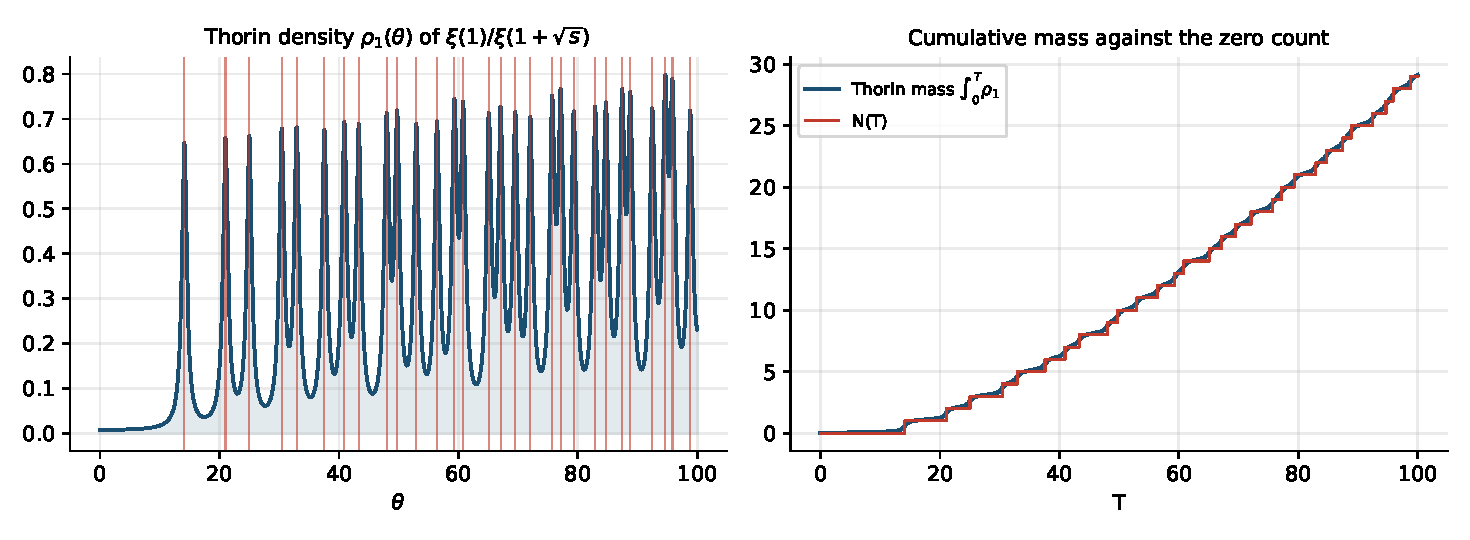
\includegraphics[width=\textwidth]{fig/bp1_density.pdf}
\caption{Left: the Thorin density $\rho_{1/2}(\theta)=v_1(\theta)/\pi$ of $T_1$ on $[0,100]$, with the ordinates of the zeros as thin vertical lines. Right: the cumulative Thorin mass $\int_0^T\rho_{1/2}$ against the zero count $N(T)$. The plot writes $\rho_1$ for $\rho_{1/2}$ and $s$ for $u$.}
\label{bp:fig:density}
\end{figure}

Because $\xi'(1)\ne0$, the Laplace transform of $T_1$ is not differentiable at the origin:
\[
\varphi_1(u)=1-\frac{\xi'}{\xi}(1)\sqrt u+O(u)=1-\Big(\sum_\rho\frac1\rho\Big)\sqrt u+O(u),\qquad u\downarrow0 .
\]
By the Tauberian theorem for Laplace transforms \cite[XIII.5]{Feller71}, $T_1$ has infinite mean and
\begin{equation}\label{bp:eq:tail}
P(T_1>x)\sim\frac{\sum_\rho\rho^{-1}}{\Gamma(\frac12)}\,x^{-1/2}=0.01303\,x^{-1/2},\qquad x\to\infty .
\end{equation}
Equivalently, near the origin the Thorin density in $z$ behaves like $\rho_{1/2}(0)/(2\sqrt z)$, which makes $\int U_1(dz)/z$ diverge. At the centre, by contrast, $\xi'(\frac12)=0$, the clock has the finite mean $\E T=\sum_ka_k^{-1}=0.0231050$, which is $\sum_{\gamma>0}\gamma^{-2}$ under RH, and the relevant constant is a sum over squared ordinates; at the basepoint one the constant is $\sum_\rho\rho^{-1}=0.0230957$, and it multiplies $\sqrt u$.

\subsection{The sine squared lemma at the basepoint one}\label{bp:sec:sin2}

At a basepoint $\alpha>1$ the sine squared lemma \eqref{eq:sin2}, applied to the canonical measure of $\log\xi$, writes $v_\alpha$ as the sum of a drift, an archimedean piece, a pole piece and a prime piece, \eqref{eq:split}. The pole piece is the image under the lemma of the measure $e^{-(\alpha-1)x}dx$ and it enters with a minus sign; the prime piece is positive. As $\alpha\downarrow1$ both diverge, the pole contribution to $-\infty$ and the prime piece to $+\infty$, because $\sum\Lambda(n)/n$ diverges (Section~\ref{sec:ch6:split}). So the lemma cannot be applied to the two pieces separately at the basepoint one. It can be applied to their difference. Throughout Section~\ref{ch:basepoint}, $\psi(y)=\sum_{n\le y}\Lambda(n)$ is Chebyshev's function, whose argument is always the real variable $y\ge1$ or the prime cutoff $X$, while at every other argument, as in $\psi(\frac32)$ or $\psi(\frac{1+i\theta}2)$, $\psi=\Gamma'/\Gamma$ is the digamma function; from here on $X$ always denotes the cutoff, not the P\'olya variable of Section~\ref{bp:sec:mellin}, and we write $\nu_1$ for the compensated prime measure of Proposition~\ref{bp:prop:sin2}, which is unrelated to the count $\nu(\sigma,T)$ of Section~\ref{ch:turing}.

\begin{proposition}\label{bp:prop:sin2}
Let $\nu_1=\sum_n\Lambda(n)n^{-1}\delta_{\log n}-\mathbf 1_{(0,\infty)}(x)\,dx$, the prime measure compensated by Lebesgue measure. For every $\theta\ne0$,
\begin{equation}\label{bp:eq:sin2one}
v_1(\theta)=\frac1{1+\theta^2}-\frac12\log\pi+\frac12\re\psi\Big(\frac{1+i\theta}2\Big)+\gamma_E+\lim_{X\to\infty}\int_0^{\log X}2\sin^2\Big(\frac{\theta x}2\Big)\nu_1(dx),
\end{equation}
that is, the limit of $\sum_{n\le X}\Lambda(n)n^{-1}2\sin^2(\frac12\theta\log n)-\big(\log X-\sin(\theta\log X)/\theta\big)$. The limit exists by the prime number theorem, and at $\theta=0$ the formula reduces to $v_1(0)=\sum_\rho\rho^{-1}$.
\end{proposition}

\begin{proof}
On the line $\re s=1$ the pole term $1/(s-1)=1/(i\theta)$ is purely imaginary, so $v_1(\theta)=\re\frac1{1+i\theta}-\frac12\log\pi+\frac12\re\psi(\frac{1+i\theta}2)+\re\frac{\zeta'}{\zeta}(1+i\theta)$. For $\re s\ge1$ with $s\ne1$, partial summation gives
\[
-\sum_{n\le X}\frac{\Lambda(n)}{n^s}+\int_1^Xy^{-s}dy=-\frac{\psi(X)-X}{X^s}-s\int_1^X(\psi(y)-y)\,y^{-s-1}dy-1,
\]
and the prime number theorem with the de la Vall\'ee Poussin error term, $\psi(y)-y=O(y\exp(-c\sqrt{\log y}))$, makes the boundary term vanish and the integral converge absolutely as $X\to\infty$, uniformly for $\re s\ge1$. For $\re s>1$ the limit is $\zeta'(s)/\zeta(s)+1/(s-1)$, and by continuity the same holds on $\re s=1$, $s\ne1$. Taking real parts at $s=1+i\theta$, where $\re\int_1^Xy^{-1-i\theta}dy=\sin(\theta\log X)/\theta$, gives $\re\frac{\zeta'}{\zeta}(1+i\theta)=\lim_X\big[-\sum_{n\le X}\Lambda(n)n^{-1}\cos(\theta\log n)+\sin(\theta\log X)/\theta\big]$. Writing $-\cos=2\sin^2-1$ and using $\sum_{n\le X}\Lambda(n)/n=\log X-\gamma_E+o(1)$, again a consequence of the prime number theorem, gives \eqref{bp:eq:sin2one}, since $\int_0^{\log X}2\sin^2(\theta x/2)dx=\log X-\sin(\theta\log X)/\theta$. At $\theta=0$ the bracket vanishes and $1-\frac12\log\pi+\frac12\psi(\frac12)+\gamma_E=1+\frac{\gamma_E}2-\frac12\log4\pi$.
\end{proof}

Table~\ref{bp:tab:sin2}, computed by \texttt{compute.py}, and Figure~\ref{bp:fig:sin2}, drawn by \texttt{figs.py}, check \eqref{bp:eq:sin2one} with primes up to $10^7$. The prime piece and the Lebesgue piece each grow like $\log X$, reaching about $16$ at $X=10^7$, and their difference converges to the exact value with an error that decreases roughly like $\log^2X/\sqrt X$, the rate the prime number theorem allows under RH.

\begin{table}[htbp]
\centering\small
\begin{tabular}{rrrrrr}
\toprule
$\theta$ & $X$ & prime piece & Lebesgue piece & formula \eqref{bp:eq:sin2one} & error\\
\midrule
5 & $10^3$ & 6.4288 & 6.9040 & 0.022767 & $-3.6\times10^{-3}$\\
5 & $10^5$ & 10.8715 & 11.3429 & 0.026558 & $1.5\times10^{-4}$\\
5 & $10^7$ & 15.8238 & 16.2955 & 0.026345 & $-6.1\times10^{-5}$\\
14.1347 & $10^3$ & 7.9028 & 6.9252 & 1.964685 & $-6.9\times10^{-2}$\\
14.1347 & $10^5$ & 12.5949 & 11.5547 & 2.027421 & $-6.4\times10^{-3}$\\
14.1347 & $10^7$ & 17.0932 & 16.0475 & 2.032931 & $-8.4\times10^{-4}$\\
30 & $10^3$ & 6.8808 & 6.9115 & 1.329190 & $5.0\times10^{-2}$\\
30 & $10^5$ & 11.4364 & 11.5191 & 1.277186 & $-1.7\times10^{-3}$\\
30 & $10^7$ & 16.0455 & 16.1267 & 1.278684 & $-2.4\times10^{-4}$\\
\bottomrule
\end{tabular}
\caption[The sine squared lemma at the basepoint one]{The sine squared lemma at the basepoint one: the prime piece $\sum_{n\le X}\Lambda(n)n^{-1}2\sin^2(\frac12\theta\log n)$, the Lebesgue piece $\log X-\sin(\theta\log X)/\theta$, the formula \eqref{bp:eq:sin2one} truncated at $X$, and its error against the exact values $v_1(\theta)=\pi\rho_{1/2}(\theta)=0.026406$, $2.033773$ and $1.278929$ at $\theta=5$, $14.1347$ and $30$.}
\label{bp:tab:sin2}
\end{table}

\begin{figure}[htbp]
\centering
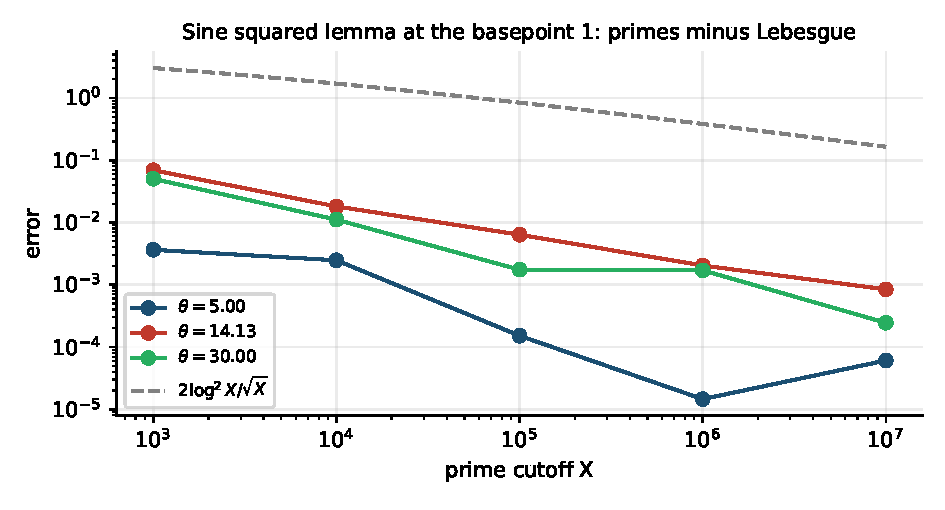
\includegraphics[width=0.72\textwidth]{fig/bp1_sin2.pdf}
\caption[Error of the compensated sine squared sum at the basepoint one]{Absolute error of the compensated sine squared sum \eqref{bp:eq:sin2one} against the prime cutoff $X$ at $\theta=5$, $14.13$ and $30$, with the reference rate $2\log^2X/\sqrt X$ (dashed).}
\label{bp:fig:sin2}
\end{figure}

So the Thorin density comes from the sine squared lemma, but its positivity does not. The lemma, applied to the compensated measure $\nu_1$, primes minus the uniform measure that represents the pole of $\zeta$, gives the arithmetic form of the density, and the existence of the sine squared integral of $\nu_1$ is the prime number theorem. Since $\nu_1$ is signed, its sine squared image is not termwise positive. Positivity comes from the zero side, Proposition~\ref{bp:prop:thorin}, through $\beta<1$, and written arithmetically it is the inequality
\[
-\re\frac{\zeta'}{\zeta}(1+it)<\frac1{1+t^2}-\frac12\log\pi+\frac12\re\psi\Big(\frac{1+it}2\Big),
\]
whose right side grows like $\frac12\log(t/2\pi)$: the inequality of Hadamard and de la Vall\'ee Poussin that underlies the proof of the prime number theorem \cite{Titchmarsh}. At the basepoint one the sine squared lemma and the prime number theorem are two readings of the same fact.

\subsection{The L\'evy form of \texorpdfstring{$\xi(1+s)$}{xi(1+s)}}\label{bp:sec:levy}

Section~\ref{bp:sec:sin2} started from the arithmetic formula for $v_1$. The sine squared lemma is designed to act one level earlier, on a L\'evy form of $\log\xi$ itself, which it converts into a Thorin form as described after \eqref{eq:sin2}, and at the basepoint one that L\'evy form exists and can be written down.

\begin{proposition}[L\'evy form]\label{bp:prop:levy}
For $\re s>0$,
\begin{equation}\label{bp:eq:levyform}
\log\frac{\xi(1+s)}{\xi(1)}=b_1s+\int_0^\infty\big(e^{-sx}-1+sx\big)\,\Pi_1(dx),
\end{equation}
with drift $b_1=-\frac12\log\pi+\frac12\psi(\frac32)+\gamma_E=\sum_\rho\rho^{-1}=0.0230957089661$ and the signed L\'evy measure
\[
\Pi_1(dx)=\Big(\frac{e^{-3x}}{1-e^{-2x}}-1\Big)\frac{dx}{x}+\sum_{n\ge2}\frac{\Lambda(n)}{n\log n}\,\delta_{\log n}(dx),
\]
the integral against the last two pieces being taken as $\lim_{X\to\infty}\int_0^{\log X}$.
\end{proposition}

\begin{proof}
Write $\xi(z)=(z-1)\pi^{-z/2}\Gamma(1+\frac z2)\zeta(z)$ and put $z=1+s$, so that $\xi(1+s)=\pi^{-(1+s)/2}\Gamma(\frac32+\frac s2)\,s\zeta(1+s)$ and $\xi(1)=\frac12$. Three classical formulas give the three pieces. The factor $\pi^{-s/2}$ contributes $-\frac s2\log\pi$. Binet's formula \cite[\S5.9]{DLMF}, $\log\Gamma(a+w)-\log\Gamma(a)=w\psi(a)+\int_0^\infty(e^{-wt}-1+wt)\frac{e^{-at}}{t(1-e^{-t})}dt$, with $a=\frac32$, $w=\frac s2$ and $t=2x$, contributes $\frac s2\psi(\frac32)$ and the density $e^{-3x}/(x(1-e^{-2x}))$. For the last factor, the Euler product gives $\log\zeta(1+s)=\sum_n\frac{\Lambda(n)}{n\log n}e^{-s\log n}$ for $\re s>0$, and Frullani's integral gives $\log s=\int_0^\infty(e^{-x}-e^{-sx})\frac{dx}x$. Their sum is $\log(s\zeta(1+s))$, which is analytic at $s=0$ with value $0$ and derivative $\gamma_E$, and subtracting the linear term puts it in the compensated form $\gamma_Es+\int(e^{-sx}-1+sx)\,x^{-1}\nu_1(dx)$, where $x^{-1}\nu_1(dx)=\sum\frac{\Lambda(n)}{n\log n}\delta_{\log n}-\frac{dx}x$. The compensated integral converges as $X\to\infty$ because the prime atoms and the measure $dx/x$ cancel at first order, by the prime number theorem in the form $\sum_{n\le X}\Lambda(n)/n=\log X-\gamma_E+o(1)$, and at zeroth order, by the logarithm of Mertens' product theorem \cite[Theorem 429]{boHardyWright}, $\sum_{p^k\le X}1/(kp^k)=\log\log X+\gamma_E+o(1)$, which does not need the prime number theorem (the logarithm of the product also contains the terms with $p\le X<p^k$, whose sum is $O(X^{-1/2})$). The drift is $\frac{d}{ds}\log\xi(1+s)|_{s=0}=\frac{\xi'}\xi(1)$.
\end{proof}

Table~\ref{bp:tab:levy}, computed by \texttt{levy.py}, checks \eqref{bp:eq:levyform} at $s=\frac12$, $1$ and $2$ with primes up to $10^7$. The prime piece and its compensator each grow like $s\log X$, reaching $28$ at $s=2$, and their difference approaches the exact value at the rate the prime number theorem allows.

\begin{table}[htbp]
\centering\small
\begin{tabular}{rrcccccc}
\toprule
$s$ & $X$ & $b_1s$ & gamma piece & primes & compensator & total & exact\\
\midrule
0.5 & $10^5$ & 0.01155 & 0.027227 & 3.40718 & 3.42845 & 0.017508 & 0.017311\\
0.5 & $10^7$ & 0.01155 & 0.027227 & 5.37344 & 5.39500 & 0.017217 & 0.017311\\
1 & $10^5$ & 0.02310 & 0.102283 & 8.41323 & 8.49224 & 0.046368 & 0.046118\\
1 & $10^7$ & 0.02310 & 0.102283 & 12.68129 & 12.76094 & 0.045729 & 0.046118\\
2 & $10^5$ & 0.04619 & 0.368975 & 19.03582 & 19.31202 & 0.138973 & 0.137917\\
2 & $10^7$ & 0.04619 & 0.368975 & 27.90836 & 28.18589 & 0.137639 & 0.137917\\
\bottomrule
\end{tabular}
\caption{The L\'evy form \eqref{bp:eq:levyform} against $\log(\xi(1+s)/\xi(1))$: the drift term, the gamma piece, the prime atoms up to $X$, their compensator, the total and the exact value.}
\label{bp:tab:levy}
\end{table}

The variable $V=V_1$ of Section~\ref{bp:sec:mellin}, the Esscher tilt by $e^{y/2}$ of the P\'olya density, has $\E e^{sV}=\xi(1+s)/\xi(1)$, so \eqref{bp:eq:levyform} has the form of a L\'evy Khintchine formula for the moment generating function of $V$, with $\Pi_1$, reflected to the negative half line by $x\mapsto-x$, in the place of the L\'evy measure. That measure is signed: the absolutely continuous part $\big(\frac{e^{-3x}}{1-e^{-2x}}-1\big)\frac1x$ is positive for $x<0.28120$, where the gamma factor dominates, and negative beyond, where the pole term $-dx/x$ dominates, and the only positive mass beyond is the prime atoms. So the uniqueness theorem for L\'evy triplets does not apply to $\Pi_1$ directly. Nor is $\Pi_1$ the signed L\'evy measure of a quasi infinitely divisible law in the sense of Lindner, Pan and Sato \cite{LPS18}, a law whose characteristic function is the quotient of two infinitely divisible ones: that would require the positive and negative parts of $\Pi_1$ to be L\'evy measures, of finite mass away from the origin, while on $(1,\infty)$ the positive part is the prime atoms and the negative part exceeds $0.94\,dx/x$, both of infinite mass, and they cancel only conditionally, which is why \eqref{bp:eq:levyform} holds only as a compensated limit. Proposition~\ref{sb:prop:qid}(3) proves that no other signed measure represents the characteristic function of $V$, so $V$ is not quasi infinitely divisible, and hence, since an infinitely divisible law is quasi infinitely divisible, not infinitely divisible. For every $\alpha>1$, by contrast, $V_\alpha$ is quasi infinitely divisible (Proposition~\ref{sb:prop:qid}(2)), so the basepoint one is exactly where the property is lost. The left panel of Figure~\ref{bp:fig:levy} shows the canonical measure $x\Pi_1(dx)$.

In the variable $\theta=\sqrt z$ the sine squared lemma \eqref{eq:sin2} reads
\[
e^{-sx}+sx-1=\frac{2x}\pi\int_0^\infty\log\Big(1+\frac{s^2}{\theta^2}\Big)\sin^2\Big(\frac{x\theta}2\Big)d\theta,\qquad\re s>0,\ x>0,
\]
and the drift converts through $\int_0^\infty\log(1+s^2/\theta^2)\,d\theta=\pi s$. Applying both to \eqref{bp:eq:levyform} and substituting $s=\sqrt u$ gives $\log\varphi_1(u)=-\int_0^\infty\log(1+u/\theta^2)\rho_{1/2}(\theta)\,d\theta$ with
\begin{equation}\label{bp:eq:conversion}
v_1(\theta)=b_1+\int_0^\infty2\sin^2\Big(\frac{x\theta}2\Big)\,x\Pi_1(dx)=b_1+A(\theta)+Q(\theta),
\end{equation}
where the drift $b_1$ is the stable part, $A(\theta)=\frac12\big[\re\psi(\frac{3+i\theta}2)-\psi(\frac32)\big]$ is the gamma piece and $Q(\theta)=\lim_{X\to\infty}\int_0^{\log X}2\sin^2(\frac{x\theta}2)\,\nu_1(dx)$ is the compensated prime piece. This is Proposition~\ref{bp:prop:sin2} again, now obtained by converting the L\'evy form rather than by manipulating $\re\xi'/\xi$; the two constant terms $-\frac12\log\pi+\gamma_E$ and $\frac12\psi(\frac32)$ combine into $b_1$, and $\frac12\re\psi(\frac{3+i\theta}2)=\frac12\re\psi(\frac{1+i\theta}2)+\frac1{1+\theta^2}$ accounts for the term $1/(1+\theta^2)$. With \texttt{levy.py} we checked that the sine squared integral of the gamma density equals the digamma expression $A(\theta)$ to ten digits at $\theta=5$, $14.1347$ and $30$ ($0.4749252962$, $0.9640604263$, $1.3367973267$).

The conversion has three readings, each visible in the right panel of Figure~\ref{bp:fig:levy}. First, the drift $b_1=\sum_\rho\rho^{-1}$ becomes the constant Thorin density $b_1/\pi$, which is the Thorin density of the positive stable one half factor $e^{-b_1\sqrt u}$. So $\varphi_1(u)=e^{-b_1\sqrt u}\exp\{-\int_0^\infty\log(1+u/\theta^2)(A+Q)(\theta)\,d\theta/\pi\}$, and the second factor is the transform of a GGC with Thorin density $(A+Q)/\pi$, because $v_1=b_1+A+Q$ attains its minimum $b_1$ only at the origin (Proposition~\ref{bp:prop:v1min}). The stable factor is the source of the tail $b_1(\pi x)^{-1/2}$ of \eqref{bp:eq:tail} and of the value $\rho_{1/2}(0)=b_1/\pi$, and it plays the role that the stable tilt plays for the floor of Section~\ref{rz:sec:floor}. At $u=(2k-1)^2$ the factorisation splits each coefficient $1/\zeta(2k)$ of Riesz's function \eqref{wr:eq:riesz}, up to an explicit factor, into a stable value and a GGC value (Section~\ref{ri:sec:ggc}). Second, the gamma factor contributes $A(\theta)\ge0$, smooth and growing like $\frac12\log(\theta/2)$: the average density of zeros. Third, the primes and the pole contribute $Q(\theta)$, which oscillates with both signs, between $-1.47$ and $1.04$ on $[0,100]$ (between $-1.29$ and $1.04$ on the window $[0,60]$ of the figure), and carries the peaks at the ordinates. Neither part converges alone; their compensated difference is the prime number theorem.

\begin{figure}[htbp]
\centering
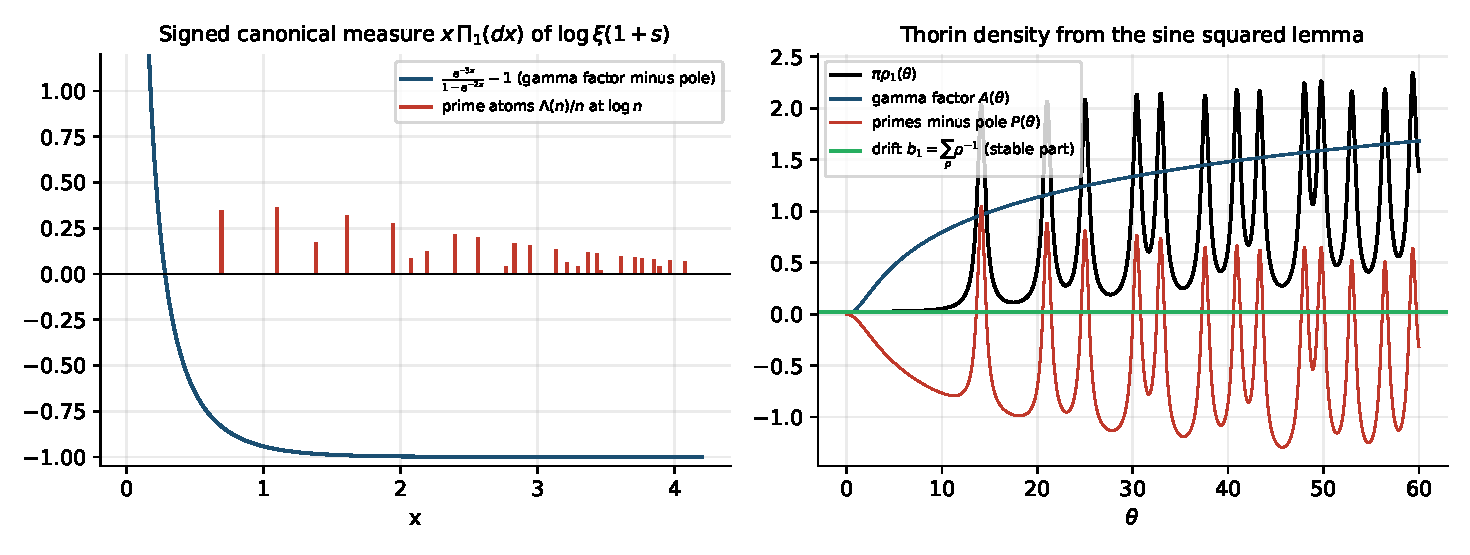
\includegraphics[width=\textwidth]{fig/bp1_levy.pdf}
\caption{Left: the signed canonical measure $x\Pi_1(dx)$ of $\log\xi(1+s)$, made of the gamma density minus the pole, $\big(\frac{e^{-3x}}{1-e^{-2x}}-1\big)dx$, which is negative beyond $x=0.28120$, and the prime atoms $\Lambda(n)/n$ at $\log n$ for $n\le60$. Right: the bracket $v_1(\theta)=\pi\rho_{1/2}(\theta)$ on $[0,60]$ assembled by the sine squared lemma from the drift $b_1$, the gamma piece $A(\theta)$ and the compensated prime piece $Q(\theta)$; the plot writes $\rho_1$ for $\rho_{1/2}$ and $P(\theta)$ for $Q(\theta)$. Drawn by \texttt{figs3.py}.}
\label{bp:fig:levy}
\end{figure}

The first reading needs $A+Q\ge0$, that is, $v_1\ge b_1$, at every height, and this holds with no hypothesis on the zeros. Near the origin $v_1$ is convex, at moderate heights a zero on the critical line is always close, and higher up every window of fixed length contains enough zeros for their Cauchy kernels to add up to more than $b_1$.

\begin{proposition}\label{bp:prop:v1min}
With no hypothesis on the zeros, $v_1(\theta)>v_1(0)=b_1$ for every real $\theta\ne0$; the proof uses a computation of the zeros below height $2000$ in ball arithmetic and, above that height, explicit bounds for the number of zeros up to a given height \cite{HSW22,Backlund}. Consequently $T_1\stackrel d=S+T_1^\circ$, where $S$ and $T_1^\circ$ are independent, $S$ is positive stable of index one half with $\E e^{-uS}=e^{-b_1\sqrt u}$, and $T_1^\circ$ is a GGC with no drift whose Thorin density in the chart $\theta=\sqrt z$ is $(v_1-b_1)/\pi=(A+Q)/\pi$.
\end{proposition}

\begin{proof}
By \eqref{bp:eq:rho1}, $v_1(\theta)=\pi\sum_\rho P_{1-\beta}(\theta-\gamma)$ is a sum of positive terms, with $\pi P_a(x)=a/(a^2+x^2)$, and $v_1$ is even, because $\xi$ is real on the real axis. We treat three ranges of $\theta\ge0$.

On $[0,13.5]$ we use convexity. Every zero has $|\gamma|\ge\gamma_1=14.134725$: the certified zeros of the next step, computed in order from the first, show that none has $0<|\gamma|<\gamma_1$, and none is real, because for $0<\sigma<1$ the alternating series $(1-2^{1-\sigma})\zeta(\sigma)=\sum_{n\ge1}(-1)^{n-1}n^{-\sigma}$ is positive while $1-2^{1-\sigma}<0$, so that $\zeta(\sigma)<0$. Since $\pi P_a''(x)=2a(3x^2-a^2)/(a^2+x^2)^3$, the kernel $P_a$ is strictly convex where $|x|>a/\sqrt3$, and for $|\theta|\le13.5$ every zero has $|\theta-\gamma|\ge\gamma_1-13.5>0.63>1/\sqrt3>(1-\beta)/\sqrt3$. So $v_1$ is strictly convex on $[-13.5,13.5]$, and, being even, it has there its unique minimum at $\theta=0$ and increases on $[0,13.5]$. By \eqref{eq:ch2:partial}, differentiated twice,
\[
v_1''(0)=-\Big(\frac{\xi'}\xi\Big)''(1)=\sum_\rho\frac{2(1-\beta)\big(3\gamma^2-(1-\beta)^2\big)}{\big((1-\beta)^2+\gamma^2\big)^3}>0 .
\]

On $[13.5,2000]$ we use the nearest zero. The script \texttt{v1min.py}, with output \texttt{v1min.json} (in the folders \texttt{riesz\_program/code} and \texttt{riesz\_program/data} of the archive), computes the first $1800$ zeros in ball arithmetic with Arb \cite{Arb}, which isolates them in order by Gram's law and Rosser's rule (Section~\ref{sec:ch5:turing}), each applied only in the range where it is known to hold \cite[Section 3]{Brent79}, so that none is missed. They reach height $2304.3$, all are simple and on the critical line, and consecutive ordinates differ by at most $\gamma_2-\gamma_1<6.8874$. Every $\theta\in[13.5,2000]$ therefore lies within $3.4437$ of an ordinate, half the largest gap, and a zero on the critical line at distance $x$ contributes $\pi P_{1/2}(x)=\frac12/(\frac14+x^2)$, which exceeds $b_1$ for $x<4.6259$. All other terms being positive,
\[
v_1(\theta)\ge\frac{1/2}{1/4+3.4437^2}>0.041,\qquad 13.5\le\theta\le2000 .
\]

For $\theta\ge2000$ we count zeros. Write $N(T)=\vartheta(T)/\pi+1+S(T)$ (Section~\ref{sec:ch5:turing}). Hasanalizade, Shen and Wong \cite[(1.7) and Corollary~1.4]{HSW22} give $|S(T)|\le2.5167$ for $0\le T\le X_0=30\,610\,046\,000$, from Platt's database of the zeros, and $|S(T)|\le0.1095\log T+0.2042\log\log T+3.0305$ for every $T\ge e$, and the smooth part $\vartheta(T)/\pi+1$ of $N(T)$ differs from $\frac T{2\pi}\log\frac T{2\pi e}+\frac78$ by at most $\frac1{50T}$ for $T\ge\frac57$ \cite[(2.7)]{HSW22}. So
\begin{multline*}
\Big|N(T)-\frac T{2\pi}\log\frac T{2\pi e}-\frac78\Big|\le E(T)\\
=\begin{cases}2.5167+\frac1{50T},&e\le T\le X_0,\\0.1095\log T+0.2042\log\log T+3.0305+\frac1{50T},&T>X_0,\end{cases}
\end{multline*}
and $E(T)<0.3\log T$ for $T>X_0$, since this holds at $X_0$ and $0.3-0.1095-0.2042/\log X_0>0$. The bound $0.112\log T+0.278\log\log T+2.510+0.2/T$ of Trudgian \cite{Trudgian}, which is often quoted, has an incomplete proof \cite{BMOR21,HSW22}. The error of Stirling's formula in the smooth part is $(\frac1{48T}+O(T^{-3}))/\pi$ \cite[Section 6.5]{Edwards}, and since the remainder of Stirling's series for $\log\Gamma(z)$ after the term $1/(12z)$ is at most $1/(90|z|^3)$ for $\re z>0$ \cite[\S5.11(ii)]{DLMF}, it is less than $0.01/T$ for $T\ge14$. The counts below use $\frac1{50T}$, as \texttt{v1min.py} does when it evaluates them; the sharper $0.01/T$, which the script also checks, would change them by less than $2\times10^{-5}$. Put $H=15$. The window $(\theta-H,\theta+H]$ holds $N(\theta+H)-N(\theta-H)$ zeros, counted with multiplicity, and since the main term has derivative $\frac1{2\pi}\log\frac T{2\pi}$, their number is at least
\[
n(\theta)=\frac H\pi\log\frac{\theta-H}{2\pi}-E(\theta-H)-E(\theta+H).
\]
While $\theta+H\le X_0$, $n$ increases, because $E$ decreases there, and $n(2000)>22.44$; for $\theta+H>X_0$, both values of $E$ are below $0.3\log(\theta+H)$, and $n(\theta)>\frac H\pi\log\frac{\theta-H}{2\pi}-0.6\log(\theta+H)>90$. So for every $\theta\ge2000$ the window holds at least $23$ zeros. Since $\xi(1-\bar s)=\overline{\xi(s)}$, the map $\rho\mapsto1-\bar\rho$ sends each zero to a zero of the same multiplicity; it keeps the ordinate and exchanges $\beta$ and $1-\beta$, so it permutes the zeros of the window, and the sum of $1-\beta$ over them is half their number. Each of them has $0<1-\beta<1$ and $|\theta-\gamma|\le H$, so its term $(1-\beta)/((1-\beta)^2+(\theta-\gamma)^2)$ in $v_1(\theta)$ exceeds $(1-\beta)/(1+H^2)$, and all other terms are positive. Hence
\[
v_1(\theta)>\frac{23}{2(1+H^2)}=\frac{23}{452}>0.05,\qquad \theta\ge2000,
\]
wherever the zeros lie. Backlund's classical constants $0.137$, $0.443$ and $4.35$, valid for $T\ge200$ \cite{Backlund}, give in the same way the increasing bound $E_B(T)=0.137\log T+0.443\log\log T+4.35+0.2/T$ in place of $E$ and at least $\frac H\pi\log\frac{\theta-H}{2\pi}-2E_B(\theta+H)$ zeros in the window, a number that increases with $\theta$ and exceeds $14.89$ at $\theta=2000$; the window then holds at least $15$ zeros, and the bound becomes $15/452>0.033$.

It remains to split $\varphi_1$. Since $\frac1\pi\int_0^\infty\log(1+u/\theta^2)\,d\theta=\sqrt u$, Proposition~\ref{bp:prop:thorin} gives
\[
\varphi_1(u)=e^{-b_1\sqrt u}\exp\Big\{-\frac1\pi\int_0^\infty\log\Big(1+\frac u{\theta^2}\Big)\big(v_1(\theta)-b_1\big)\,d\theta\Big\},\qquad u\ge0,
\]
where the integral is finite because $0\le v_1-b_1\le v_1$ and $\int_0^\infty\log(1+u/\theta^2)\,v_1(\theta)\,d\theta=-\pi\log\varphi_1(u)$ is finite by Theorem~\ref{thm:poisson} at $\alpha=1$. The first factor is the Laplace transform of the positive stable law of index one half with density $\frac{b_1}{2\sqrt\pi}t^{-3/2}e^{-b_1^2/(4t)}$. The image $U_1^\circ$ of $\pi^{-1}(v_1-b_1)\,d\theta$ under $\theta\mapsto\theta^2=z$ is a positive measure with $\int\log(1+u/z)\,U_1^\circ(dz)<\infty$, which is equivalent to the integrability condition in \eqref{eq:ch3:ggc}, so the second factor is the Laplace transform of a GGC $T_1^\circ$ with no drift. A product of Laplace transforms is the transform of the sum of independent variables, so $T_1\stackrel d=S+T_1^\circ$, and $v_1-b_1=A+Q$ by \eqref{bp:eq:conversion}.
\end{proof}

The factorisation separates the tail of $T_1$ from the rest of its law. The stable summand carries the infinite mean and the whole tail: $P(S>t)\sim b_1/\sqrt{\pi t}$ is the tail \eqref{bp:eq:tail} of $T_1$, while $T_1^\circ$ has finite mean and infinite variance. The Laplace exponent of $T_1^\circ$ is $\log(\xi(1+\sqrt u)/\xi(1))-b_1\sqrt u=\frac12(\log\xi)''(1)\,u+O(u^{3/2})$ as $u\downarrow0$, so that
\[
\E T_1^\circ=\frac12(\log\xi)''(1)=-\frac12\sum_\rho\rho^{-2}=0.0230772,
\]
and its Thorin density $(v_1-b_1)/\pi$ vanishes at the origin to exactly second order, since $v_1$ is even and $v_1''(0)>0$; for instance $v_1(1)-b_1=1.12\times10^{-4}$ and $v_1(5)-b_1=3.31\times10^{-3}$. Near $z=0$ the Thorin measure $U_1^\circ$ therefore has a density of exact order $\sqrt z$, and the variance $\int z^{-2}\,U_1^\circ(dz)$ is infinite. On $[13.5,2000]$ the smallest value of $v_1$ on the grid of step $0.02$ of \texttt{v1min.py} is $0.11326$, at $\theta=17.5$ in the valley between the first two ordinates, about five times $b_1$. An independent check, \texttt{v1\_grid\_mp.py} in the folder \texttt{repro}, evaluates the arithmetic form of $v_1$ with \texttt{mpmath} \cite{mpmath} to $25$ digits on the grid of step $0.005$ in $(0,2100]$. It finds $v_1>b_1$ at all $420000$ points, the smallest excess being $2.8\times10^{-9}$, at $\theta=0.005$, which is $0.005^2(v_1(1)-b_1)$ to two digits, as the vanishing to second order predicts; the smallest value on $[13.5,2000]$ is $0.1132554$, at $\theta=17.495$. The first $1850$ zeros, computed with \texttt{mpmath} by \texttt{zeros\_mp.py}, agree with those of Arb to double precision.

The same construction applies at every basepoint above one. For every $\alpha\ge1$ it gives the L\'evy form of $\log(\xi(\alpha+s)/\xi(\alpha))$ with drift $b_\alpha=\frac{\xi'}\xi(\alpha)$ and
\begin{gather*}
x\Pi_\alpha(dx)=\Big(\frac{e^{-(\alpha+2)x}}{1-e^{-2x}}-e^{-(\alpha-1)x}\Big)dx+\sum_n\frac{\Lambda(n)}{n^\alpha}\,\delta_{\log n}(dx),\\
v_\alpha(\theta)=b_\alpha+\int_0^\infty2\sin^2\Big(\frac{x\theta}2\Big)x\Pi_\alpha(dx),
\end{gather*}
which for $\alpha>1$ is \eqref{eq:split}. For $\alpha>1$ every piece converges on its own, and the pole contribution is the finite negative term $-\theta^2/((\alpha-1)((\alpha-1)^2+\theta^2))$. Expanding $1/(e^{2x}-1)=\sum_{k\ge1}e^{-2kx}$ in the archimedean piece of \eqref{eq:split}, and writing $q_c(\theta)=\int_0^\infty(1-\cos\theta x)e^{-cx}\,dx=\theta^2/(c(c^2+\theta^2))$, gives
\begin{equation}\label{bp:eq:excess}
v_\alpha(\theta)-b_\alpha=\sum_{k\ge1}q_{\alpha+2k}(\theta)-q_{\alpha-1}(\theta)+\sum_{n\ge2}\frac{\Lambda(n)}{n^\alpha}\big(1-\cos(\theta\log n)\big),\qquad\alpha>1 .
\end{equation}
Only the pole term is negative. Near the origin $q_c(\theta)\sim\theta^2/c^3$, and the pole term outweighs the gamma terms when $\alpha<7.789$, where $\frac18\zeta(3,\frac\alpha2+1)=(\alpha-1)^{-3}$; below that basepoint the arithmetic form needs the primes to keep $v_\alpha-b_\alpha$ positive near the origin. On the zero side positivity there is again convexity, and the factorisation of Proposition~\ref{bp:prop:v1min} holds at every basepoint above one.

\begin{proposition}\label{bp:prop:valpha}
With no hypothesis on the zeros, $v_\alpha(\theta)>v_\alpha(0)=b_\alpha$ for every $\alpha\ge1$ and every real $\theta\ne0$; the proof uses the zeros below height $2000$ of Proposition~\ref{bp:prop:v1min}, the explicit bounds of \cite{HSW22} for the number of zeros above that height, and a computation in ball arithmetic. Consequently, for every $\alpha\ge1$, $T_\alpha\stackrel d=S_\alpha+T_\alpha^\circ$, where $S_\alpha$ and $T_\alpha^\circ$ are independent, $S_\alpha$ is positive stable of index one half with $\E e^{-uS_\alpha}=e^{-b_\alpha\sqrt u}$, which is the law of the first passage time of Brownian motion to the level $b_\alpha/\sqrt2$, and $T_\alpha^\circ$ is a GGC with no drift, with Thorin density $(v_\alpha-b_\alpha)/\pi$ in the chart $\theta=\sqrt z$ and mean $\E T_\alpha^\circ=\frac12(\log\xi)''(\alpha)$.
\end{proposition}

\begin{proof}
At $\alpha=1$ this is Proposition~\ref{bp:prop:v1min}, so let $\alpha>1$. Since $v_\alpha$ is even, it suffices to take $\theta>0$. A zero $\rho=\beta+i\gamma$ contributes $a/(a^2+(\theta-\gamma)^2)$ to $v_\alpha(\theta)$, with $a=\alpha-\beta\in(\alpha-1,\alpha)$, and we put $\theta_0(\alpha)=\gamma_1-\alpha/\sqrt3$. Four steps cover all $\alpha>1$.

Near the origin, for $\alpha\le9$, we use convexity. If $0<\theta\le\theta_0(\alpha)$, every zero has $|\theta-\gamma|\ge\gamma_1-\theta\ge\alpha/\sqrt3>a/\sqrt3$, so, as in the proof of Proposition~\ref{bp:prop:v1min}, $v_\alpha$ is strictly convex on $[-\theta_0(\alpha),\theta_0(\alpha)]$, and $v_\alpha(\theta)>v_\alpha(0)$ there. Since $\theta_0(9)=8.94>0$, it remains to treat $\theta>\theta_0(\alpha)$ for $\alpha\le9$, and every $\theta>0$ for $\alpha>9$.

For $1<\alpha\le3$ we use the zeros. Here $\theta_0(\alpha)\ge\theta_0(3)=12.40$ and $\gamma_1-12.40<3.4437$, so by the computation in the proof of Proposition~\ref{bp:prop:v1min} every $\theta\in[\theta_0(\alpha),2000]$ lies within $3.4437$ of the ordinate of a zero on the critical line, whose term exceeds $r(\alpha)=(\alpha-\frac12)/((\alpha-\frac12)^2+3.4437^2)$. For $\theta\ge2000$ the window $(\theta-15,\theta+15]$ holds at least $20$ zeros, the sum of $a$ over them is $\alpha-\frac12$ times their number, and each term exceeds $a/(\alpha^2+225)$, so that $v_\alpha(\theta)>w(\alpha)=20(\alpha-\frac12)/(\alpha^2+225)$. The functions $r$ and $w$ increase on $[1,3]$, and so does $b_\alpha$, whose derivative $\sum_\rho(\gamma^2-a^2)/(a^2+\gamma^2)^2$ is positive for $\alpha<\gamma_1$. It therefore suffices that $r(\alpha_k)>b_{\alpha_{k+1}}$ and $w(\alpha_k)>b_{\alpha_{k+1}}$ at the points $\alpha_k=1+k/256$, and in ball arithmetic the smallest margins are $0.0180$ and $0.0209$.

For $3\le\alpha\le7$ we use the primes. Adding and subtracting $q_\alpha(\theta)$ in \eqref{bp:eq:excess}, dropping the prime terms and using $q_c(\theta)<1/c$ gives
\begin{align*}
v_\alpha(\theta)-b_\alpha>L(\alpha,\theta)&=\sum_{k\ge0}q_{\alpha+2k}(\theta)-\frac1\alpha-\frac1{\alpha-1}\\
&=\frac12\Big[\re\psi\Big(\frac{\alpha+i\theta}2\Big)-\psi\Big(\frac\alpha2\Big)\Big]-\frac1\alpha-\frac1{\alpha-1},
\end{align*}
which increases in $\theta$. Since $|\psi'(z)|\le\psi'(\re z)$ and $\psi'(x)\le1/x+1/x^2$ for $x>0$, $|\partial L/\partial\alpha|\le M(\alpha)=1/\alpha+3/\alpha^2+1/(\alpha-1)^2$, which decreases in $\alpha$. It therefore suffices that $L(\alpha_k,\theta_0(\alpha_{k+1}))>M(\alpha_k)/256$ at the points $\alpha_k=3+k/256$ of $[3,7]$; the smallest margin is $0.0228$, at $\alpha=7$, and the same check succeeds up to $\alpha=7.707$.

For $\alpha\ge7$ the gamma terms suffice. Since $q_c(\theta)$ decreases in $c$, $\sum_{k\ge1}q_{\alpha+2k}(\theta)\ge\frac12\int_{\alpha+2}^\infty q_c(\theta)\,dc=\frac14\log(1+\theta^2/(\alpha+2)^2)$, so with $A=\alpha+2$, $B=\alpha-1$ and $s=\theta^2$,
\[
v_\alpha(\theta)-b_\alpha\ge\Phi_\alpha(s)=\frac14\log\Big(1+\frac s{A^2}\Big)-\frac s{B(B^2+s)} .
\]
Here $\Phi_\alpha(0)=0$, and $\Phi_\alpha'(s)=1/(4(A^2+s))-B/(B^2+s)^2$ is nonnegative exactly when $(B^2+s)^2\ge4B(A^2+s)$, the two sides differing by a function that increases in $s$ when $B\ge2$. For $\alpha\ge9$ they are in this order already at $s=0$, because $B^3-4A^2=(\alpha-1)^3-4(\alpha+2)^2$ is $28$ at $\alpha=9$ and increases beyond, so $\Phi_\alpha(s)>0$ for every $s>0$, and no zero enters. For $7\le\alpha\le9$ and $\theta>\theta_0(\alpha)\ge\theta_0(9)$, we have $s>s_9=\theta_0(9)^2=79.90$, $6\le B\le8$ and $A\le11$, so $(B^2+s_9)^2\ge(36+s_9)^2>32(121+s_9)\ge4B(A^2+s_9)$; hence $\Phi_\alpha$ increases on $[s_9,\infty)$, where $\Phi_\alpha(s_9)\ge\frac14\log(1+s_9/121)-s_9/(6(36+s_9))>0.0118$.

The script \texttt{valpha\_min.py} in the folder \texttt{repro} carries out the checks of the last three steps in ball arithmetic with Arb \cite{Arb}, computing $b_\alpha$ from $\zeta(\alpha)$ and $\zeta'(\alpha)$. The factorisation follows from the inequality as in the proof of Proposition~\ref{bp:prop:v1min}, Theorem~\ref{thm:poisson} giving $\int_0^\infty\log(1+u/\theta^2)\,v_\alpha(\theta)\,d\theta<\infty$, and the mean is the coefficient of $u$ in $\log(\xi(\alpha+\sqrt u)/\xi(\alpha))-b_\alpha\sqrt u=\frac12(\log\xi)''(\alpha)\,u+O(u^{3/2})$.
\end{proof}

As at the basepoint one, $v_\alpha-b_\alpha$ starts as $c(\alpha)\theta^2$, with $c(\alpha)=-\frac12(\xi'/\xi)''(\alpha)>0$, so at every basepoint above one the Thorin density of $T_\alpha^\circ$ vanishes to second order at the origin, $T_\alpha^\circ$ has finite mean and infinite variance, and $S_\alpha$ carries the whole tail $P(T_\alpha>t)\sim b_\alpha/\sqrt{\pi t}$. The two summands move very differently with the basepoint. From $\alpha=1$ to $\alpha=9$ the drift $b_\alpha$ grows from $0.0230957$ to $0.3567685$, while the mean of the remainder falls only slowly, $\E T_\alpha^\circ$ being $0.0230772$, $0.0230425$, $0.0229942$, $0.0228577$, $0.0224351$, $0.0211082$ and $0.0176077$ at $\alpha=1$, $1.25$, $1.5$, $2$, $3$, $5$ and $9$; at the last six basepoints $c(\alpha)$ is $1.66$, $2.20$, $3.25$, $5.15$, $7.85$ and $8.85\times10^{-4}$ (computed by \texttt{valpha\_min.py}).

For $\alpha<1$ the Euler product no longer converges near $\re s=\alpha$, and the prime atoms $\Lambda(n)n^{-\alpha}$ can be compensated only if the primes are well enough distributed. So the route from the L\'evy form through the sine squared lemma computes the Thorin measure unconditionally on $\alpha\ge1$, the region where it is positive unconditionally; Section~\ref{bp:sec:below} shows exactly how far below the basepoint one it extends.

\subsection{Below the basepoint one}\label{bp:sec:below}

The construction of Section~\ref{bp:sec:levy} can be written down for any basepoint $\alpha=1-\varepsilon$ with $0<\varepsilon<\frac12$, and the question is whether it converges. Formally nothing changes except the pole term, which now grows: with $b_\alpha=\frac{\xi'}\xi(\alpha)$,
\[
x\Pi_\alpha(dx)=\frac{e^{-(\alpha+2)x}}{1-e^{-2x}}\,dx\;+\;\Big(\sum_n\frac{\Lambda(n)}{n^{\alpha}}\,\delta_{\log n}(dx)-e^{\varepsilon x}\,dx\Big),
\]
and the converted Thorin density would be $\pi^{-1}$ times
\begin{equation}\label{bp:eq:below}
b_\alpha+A_\alpha(\theta)+\lim_{X\to\infty}\Big[\sum_{n\le X}\frac{\Lambda(n)}{n^\alpha}\,2\sin^2\Big(\frac{\theta\log n}2\Big)-\int_0^{\log X}2\sin^2\Big(\frac{\theta x}2\Big)e^{\varepsilon x}dx\Big],
\end{equation}
with $A_\alpha(\theta)=\frac12\big[\re\psi(\frac{\alpha+2+i\theta}2)-\psi(\frac{\alpha+2}2)\big]$. The prime piece and the pole piece now each grow like $X^\varepsilon/\varepsilon$, and whether their difference converges is a question about how well $\psi(y)$ is approximated by $y$.

\begin{proposition}\label{bp:prop:below}
Let $\Theta=\sup\{\re\rho\}$ over the nontrivial zeros and let $\frac12<\alpha<1$.
\begin{enumerate}
\item If $\Theta<\alpha$, the L\'evy form $\log\frac{\xi(\alpha+s)}{\xi(\alpha)}=b_\alpha s+\int_0^\infty(e^{-sx}-1+sx)\Pi_\alpha(dx)$ holds for $\re s>0$, the compensated limit converging, and the sine squared lemma converts it into \eqref{bp:eq:below}, which then equals $v_\alpha(\theta)$ and is positive. The error of the compensated sum with prime cutoff $X$ is $O(X^{\Theta-\alpha+\delta})$ for every $\delta>0$.
\item Conversely, if the L\'evy form holds for $\re s>0$, then $\xi(\alpha+s)$ has no zeros with $\re s>0$, so $\Theta\le\alpha$.
\end{enumerate}
\end{proposition}

\begin{proof}
If $\Theta<\alpha$, the explicit formula gives $\psi(y)-y=O(y^{\Theta+\delta})$ for every $\delta>0$ \cite{Titchmarsh}. Then the Stieltjes integral $\int_1^\infty y^{-w}\,d(\psi(y)-y)$, which equals $-\frac{\zeta'}{\zeta}(w)-\frac1{w-1}$ for $\re w>1$, converges after one integration by parts for $\re w>\Theta$ and provides the analytic continuation there, with tail beyond $X$ of order $X^{\Theta-\re w+\delta}$. Taking $w=\alpha+s$ with $\re s\ge0$ and integrating twice in $s$ from $s=0$ gives the compensated L\'evy form, the gamma and polynomial factors being handled exactly as in Proposition~\ref{bp:prop:levy}. For fixed $\theta$ the sine squared lemma may be applied under the limit, because the compensated measure integrated against $2\sin^2(\theta x/2)$ is a combination of the same convergent Stieltjes integrals at $w=\alpha$ and $w=\alpha\pm i\theta$. Positivity follows from the Poisson form of Proposition~\ref{prop:struct}, as in Proposition~\ref{bp:prop:thorin}, with widths $\alpha-\beta>0$. Conversely, suppose the L\'evy form holds for $\re s>0$. Write $\nu_\alpha$ for the bracket in $x\Pi_\alpha$, so that the compensated part of the right side is the limit of $\int_0^{\log X}(e^{-sx}-1+sx)\,x^{-1}\nu_\alpha(dx)$; its part over $[0,1]$ is an entire function of $s$. For real $s>1-\alpha$ the integral $\int_1^\infty e^{-sx}x^{-1}\nu_\alpha(dx)$ converges absolutely, so the convergence of the compensated limit at two such values of $s$ gives that of $\int_1^{\log X}\nu_\alpha(dx)$ and of $\int_1^{\log X}x^{-1}\nu_\alpha(dx)$. The function $y\mapsto\int_1^y\nu_\alpha(dx)$ is therefore bounded on $[1,\infty)$, and one integration by parts against it shows that $\int_1^{\log X}e^{-sx}x^{-1}\nu_\alpha(dx)$ converges uniformly on compact subsets of $\re s>0$. So the compensated limit converges locally uniformly, the right side of the L\'evy form is analytic in $\re s>0$, hence so is $\log\xi(\alpha+s)$, and $\xi(\alpha+s)$ cannot vanish there.
\end{proof}

So the extension to $\xi(1-\varepsilon+s)$ exists exactly when $\zeta$ has no zeros in the half plane $\re s>1-\varepsilon$, up to the boundary case $\Theta=1-\varepsilon$. At the basepoint one the convergence of the compensated sum was the prime number theorem; at the basepoint $1-\varepsilon$ it is the estimate $\psi(y)-y=O(y^{1-\varepsilon+\delta})$, which is the zero free half plane $\re s>1-\varepsilon$; and as $\varepsilon\uparrow\frac12$ it is $\psi(y)-y=O(y^{1/2+\delta})$, which is RH. The L\'evy form route therefore reaches exactly as far as the zero free region does. It is an arithmetic restatement of step~7 of the path in Table~\ref{tab:ch25:path}, not a way around it.

Table~\ref{bp:tab:below}, computed by \texttt{below.py}, evaluates \eqref{bp:eq:below} with primes up to $10^7$ at $\theta=\gamma_1$ and compares it with $v_\alpha(\gamma_1)$ computed directly. On the range of the computation the primes behave as RH predicts, $\psi(y)-y=O(y^{1/2}\log^2y)$, so the errors should decay like $X^{1/2-\alpha}$, and they do (Figure~\ref{bp:fig:below}, left): the decay is fast at $\alpha=0.9$, slow at $\alpha=0.6$, where the prime and pole pieces are about $1500$ and their difference is still wrong by about $2$, and absent at the centre. At $\alpha=\frac12$ and $\theta=\gamma_1$ the compensated sum grows like $\log X$ (Figure~\ref{bp:fig:below}, right), which is the atom $\delta_{\gamma_1}$ of the RH measure forming as the cutoff increases; away from the zeros it oscillates without converging. The rate of convergence is thus itself a diagnostic: the exponent in $X^{\Theta-\alpha}$ measures the largest real part of a zero, although only up to the range of $X$ that can be computed, so it can never certify $\Theta$.

\begin{table}[htbp]
\centering\small
\begin{tabular}{cccccc}
\toprule
$\alpha$ & $X$ & prime piece & pole piece & formula \eqref{bp:eq:below} & $v_\alpha(\gamma_1)$\\
\midrule
1 & $10^7$ & 17.093 & 16.047 & 2.03293 & 2.03377\\
0.9 & $10^5$ & 23.250 & 21.754 & 2.50194 & 2.52704\\
0.9 & $10^7$ & 41.281 & 39.765 & 2.52202 & 2.52704\\
0.75 & $10^5$ & 70.611 & 67.856 & 3.79129 & 4.01691\\
0.75 & $10^7$ & 219.869 & 216.972 & 3.93394 & 4.01691\\
0.6 & $10^5$ & 257.280 & 251.510 & 6.84001 & 10.00677\\
0.6 & $10^7$ & 1537.254 & 1530.446 & 7.87829 & 10.00677\\
0.5 & $10^5$ & 653.402 & 642.998 & 11.497 & $+\infty$ (a zero)\\
0.5 & $10^7$ & 6114.332 & 6099.976 & 15.449 & $+\infty$ (a zero)\\
\bottomrule
\end{tabular}
\caption{The compensated sine squared formula \eqref{bp:eq:below} below the basepoint one at $\theta=\gamma_1$, with primes up to $X$, against the directly computed $v_\alpha(\gamma_1)=\re(\xi'/\xi)(\alpha+i\gamma_1)$; at $\alpha=\frac12$ the point $\frac12+i\gamma_1$ is a zero.}
\label{bp:tab:below}
\end{table}

\begin{figure}[htbp]
\centering
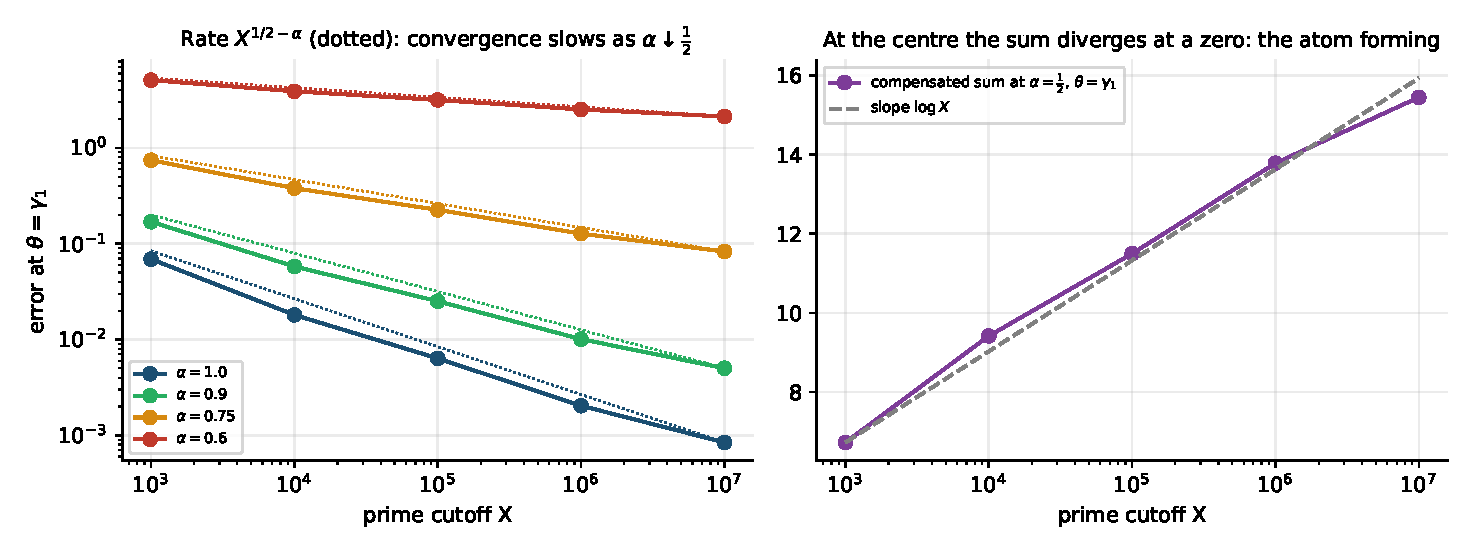
\includegraphics[width=\textwidth]{fig/bp1_below.pdf}
\caption{Left: absolute error of the compensated formula \eqref{bp:eq:below} at $\theta=\gamma_1$ against the prime cutoff $X$ for $\alpha=1$, $0.9$, $0.75$ and $0.6$, with the rates $X^{1/2-\alpha}$ (dotted). Right: at the centre, $\alpha=\frac12$, the compensated sum at the first ordinate grows like $\log X$ (dashed line), the atom of the RH measure forming. Drawn by \texttt{figs4.py}.}
\label{bp:fig:below}
\end{figure}

The slow convergence can be explained exactly, term by term over the zeros. Writing the tail of the compensated sum beyond $X$ as a Stieltjes integral against $d(\psi(y)-y)$ and inserting the explicit formula $\psi(y)=y-\sum_\rho y^\rho/\rho-\log2\pi-\frac12\log(1-y^{-2})$ \cite[Chapter~17]{Davenport} gives, for $\Theta<\alpha$ and $X$ not a prime power,
\begin{multline}\label{bp:eq:errformula}
\text{(formula \eqref{bp:eq:below} at cutoff }X)-v_\alpha(\theta)\\
=\sum_\rho\Big[-\frac{X^{\rho-\alpha}}{\rho-\alpha}+\frac{X^{\rho-\alpha+i\theta}}{2(\rho-\alpha+i\theta)}+\frac{X^{\rho-\alpha-i\theta}}{2(\rho-\alpha-i\theta)}\Big]+O(X^{-1-\alpha}),
\end{multline}
the sum taken over conjugate pairs. Every term has size $X^{\beta-\alpha}$, which makes the rate $X^{\Theta-\alpha}$ visible term by term, and at $\theta=\gamma$ the third term has denominator $\beta-\alpha$, so under RH it approaches $X^{1/2-\alpha}/(1-2\alpha)$ and at the centre it becomes the $\log X$ growth of Figure~\ref{bp:fig:below}. Table~\ref{bp:tab:err}, computed by \texttt{errformula.py}, compares the observed error with \eqref{bp:eq:errformula} truncated to the $1700$ zeros below height $2198$, and shows the error left after subtracting it. The explicit formula accounts for the error to four or five decimal places for $\alpha\ge0.75$ and to three at $\alpha=0.6$, and the hybrid of primes up to $X$ plus the first $1700$ zeros reduces the error of the primes alone by factors between about $700$ and $11000$: at $\alpha=0.6$ the error falls from $2.13$ to $7.7\times10^{-4}$.

\begin{table}[htbp]
\centering\small
\begin{tabular}{ccccc}
\toprule
$\alpha$ & $X$ & observed error & predicted by \eqref{bp:eq:errformula} & error after correction\\
\midrule
1 & $10^5$ & $-6.352\times10^{-3}$ & $-6.349\times10^{-3}$ & $-2.9\times10^{-6}$\\
1 & $10^7$ & $-8.419\times10^{-4}$ & $-8.431\times10^{-4}$ & $1.2\times10^{-6}$\\
0.9 & $10^7$ & $-5.014\times10^{-3}$ & $-5.020\times10^{-3}$ & $6.1\times10^{-6}$\\
0.75 & $10^7$ & $-8.297\times10^{-2}$ & $-8.304\times10^{-2}$ & $6.8\times10^{-5}$\\
0.6 & $10^5$ & $-3.1668$ & $-3.1665$ & $-2.9\times10^{-4}$\\
0.6 & $10^7$ & $-2.1285$ & $-2.1292$ & $7.7\times10^{-4}$\\
\bottomrule
\end{tabular}
\caption{The error of the compensated sum \eqref{bp:eq:below} at $\theta=\gamma_1$ with primes up to $X$, its prediction from the explicit formula \eqref{bp:eq:errformula} over the first $1700$ zeros, and what remains after subtracting the prediction.}
\label{bp:tab:err}
\end{table}

This also sharpens the logic of Proposition~\ref{bp:prop:below}. A zero with $\beta>\alpha$ would contribute a term of size $X^{\beta-\alpha}$ that grows with the cutoff, so the compensated sum at the basepoint $\alpha$ would diverge, and the size and phase of that growth would locate the zero. The hybrid formula is a zero detector with the same structure as Turing's method (Section~\ref{sec:ch5:turing}): primes up to $X$ and zeros up to height $T$ must balance to within the tail of both.

The role of the pole also changes below the basepoint one. If instead of compensating one continues the pole contribution analytically, its value at $\alpha=1-\varepsilon$ is $\re\frac1{-\varepsilon+i\theta}+\frac1\varepsilon=\frac{\theta^2}{\varepsilon(\varepsilon^2+\theta^2)}$, which is positive, since the pole now lies to the right of the basepoint. The single negative term of the decomposition \eqref{eq:split} above the basepoint one has become positive, and the difficulty has moved entirely into the prime sum, which no longer converges on its own. Below the line $\re s=1$, therefore, the negativity that RH must control is carried by the primes, not by the pole.

\subsection{The minimum at the origin below the basepoint one}\label{sec:dbeta:comp}

Propositions~\ref{bp:prop:v1min} and \ref{bp:prop:valpha} put the minimum of $v_\alpha$ at the origin for every $\alpha\ge1$, with no hypothesis on the zeros. Below the basepoint one the margin at the origin vanishes linearly, $b_\alpha\approx(\alpha-\frac12)(\log\xi)''(\frac12)$, and Table~\ref{bp:tab:alpha} found the minimum at the origin on a window by computation. This subsection proves it on the range of heights where the zeros are known to lie on the critical line, up to $\frac{1+\sqrt2}2$ below its top, for every basepoint $\alpha\in(\frac12,7.35]$, and shows that RH is equivalent to it at every height for every $\alpha\in(\frac12,1)$. The tool is a comparison across vertical lines, from the first author's note on the Dirichlet beta function \cite{P26beta}. It uses only the Hadamard product, the functional equation and an elementary bound on one line to the right of $\re s=1$, so it applies equally to the completed $L$ functions of Section~\ref{ch:chi12}. We state it for $f=\xi$, for $f=\xi(\cdot,\chi_4)$ of Section~\ref{sec:dbeta:beta} and for $f=\xi(\cdot,\chi_{12})$ of Section~\ref{sec:ch16:eta}, and write $v_\alpha(\theta)=\re(f'/f)(\alpha+i\theta)$, $b_\alpha=v_\alpha(0)=(f'/f)(\alpha)$ and $V_f=(\log f)''(\frac12)$. For the two $L$ functions the result is the full analogue of Proposition~\ref{bp:prop:valpha}.

Each $f$ is entire of order one, real on the real axis, with $f(s)=f(1-s)$ and no real zeros. Its zeros therefore come in groups: a zero $\frac12+i\gamma$ on the critical line, or a pair $\frac12\pm\delta+i\gamma$ with $0<\delta<\frac12$. At resolution $\varepsilon=\alpha-\frac12$ and offset $u=\theta-\gamma$, a zero on the line contributes $\varepsilon/(\varepsilon^2+u^2)$ to $v_\alpha(\theta)$, and a pair contributes
\begin{equation}\label{eq:dbeta:pair}
k_\delta(\varepsilon,u)=\frac{\varepsilon-\delta}{(\varepsilon-\delta)^2+u^2}+\frac{\varepsilon+\delta}{(\varepsilon+\delta)^2+u^2}=\frac{2\varepsilon(w+c)}{(w+c)^2+\kappa^2},
\end{equation}
where $w=\varepsilon^2$, $c=u^2-\delta^2$ and $\kappa=2\delta|u|$, since the numerator of the sum is $2\varepsilon(\varepsilon^2+u^2-\delta^2)$ and its denominator is $(\varepsilon^2+\delta^2+u^2)^2-4\varepsilon^2\delta^2=(w+c)^2+\kappa^2$. The pair contribution is negative exactly when $u^2<\delta^2-\varepsilon^2$, which is Proposition~\ref{prop:signature}(ii). The sum over the groups converges absolutely, since $\sum_\rho|\rho|^{-2}<\infty$. So $v_\alpha(\theta)/(\alpha-\frac12)$ is the sum over the groups of the ratios $1/(w+u^2)$ for the zeros on the line and
\[
r_\delta(w,u)=\frac{k_\delta(\varepsilon,u)}\varepsilon=2\re\frac1{w+c+i\kappa}
\]
for the pairs, as functions of $w=(\alpha-\frac12)^2$. The ratio of a zero on the line decreases in $w$; that of a pair need not.

\begin{lemma}[Comparison]\label{lem:dbeta:comp}
Let $0<\delta<\frac12$ and let $u$ be real. As a function of $w>0$, the ratio $r_\delta(w,u)$
\begin{enumerate}
\item[(a)] is nonincreasing on $(0,\infty)$ if $|u|\ge(1+\sqrt2)\delta$;
\item[(b)] is nonincreasing on $[2\delta^2,\infty)$ for every $u$, in particular on $w\ge\frac12$, that is for $\alpha\ge\frac12+\frac1{\sqrt2}$, whatever $\delta$;
\item[(c)] if $0<|u|<(1+\sqrt2)\delta$, increases exactly on the interval $\max\big(0,2\delta^2-(|u|+\delta)^2\big)<w<2\delta^2-(|u|-\delta)^2$, which begins at $0$ if and only if $|u|\ge(\sqrt2-1)\delta$; at $u=0$ it equals $2/(w-\delta^2)$, which has a pole at $w=\delta^2$.
\end{enumerate}
In particular the constant $1+\sqrt2$ in (a) cannot be lowered.
\end{lemma}

\begin{proof}
For $u\ne0$, $\partial_wr_\delta=-2\re(w+c+i\kappa)^{-2}=-2\big((w+c)^2-\kappa^2\big)/\big((w+c)^2+\kappa^2\big)^2$, which is positive exactly when $-\kappa<w+c<\kappa$, that is when $2\delta^2-(|u|+\delta)^2<w<2\delta^2-(|u|-\delta)^2$, since $-\kappa-c=2\delta^2-(|u|+\delta)^2$ and $\kappa-c=2\delta^2-(|u|-\delta)^2$. The right end is at most $2\delta^2$, which gives (b) for $u\ne0$; it is positive exactly when $\big||u|-\delta\big|<\sqrt2\delta$, that is when $|u|<(1+\sqrt2)\delta$, which gives (a) and the first part of (c); and the left end is at most $0$ exactly when $|u|+\delta\ge\sqrt2\delta$. At $u=0$, $c=-\delta^2$ and $\kappa=0$, and $2/(w-\delta^2)$ decreases on $w>\delta^2$, which completes (b). Finally $2\delta^2<\frac12$ because $\delta<\frac12$.
\end{proof}

So for $(\sqrt2-1)\delta\le|u|<(1+\sqrt2)\delta$ the ratio of a pair increases from $w=0$ up to $w=2\delta^2-(|u|-\delta)^2$, while for $0<|u|<(\sqrt2-1)\delta$ it first decreases and then increases up to that point; in both cases it decreases beyond it. Summing the lemma over the groups gives the comparison.

\begin{theorem}[Comparison across vertical lines]\label{thm:dbeta:comp}
Let $\frac12<\alpha<\alpha'$ and let $\theta$ be real. Suppose that every zero $\frac12+\delta+i\gamma$ of $f$ with $\delta>(\alpha-\frac12)/\sqrt2$ satisfies $|\theta-\gamma|\ge(1+\sqrt2)\delta$. Then
\[
\frac{v_\alpha(\theta)}{\alpha-\frac12}\ \ge\ \frac{v_{\alpha'}(\theta)}{\alpha'-\frac12}.
\]
The hypothesis holds at every $\theta$ under RH for $\xi$, or GRH for $\chi_4$ or $\chi_{12}$; at every $\theta$ when $\alpha\ge\frac12+\frac1{\sqrt2}$, with no hypothesis; and at every $\theta$ with $|\theta|\le H_0-\frac{1+\sqrt2}2$, where $H_0$ is a height below which every zero of $f$ is known to lie on the critical line: $H_0=3\times10^{12}$ for $\xi$ \cite{PT21}, and $H_0=10^8/q$ for $\xi(\cdot,\chi_q)$, that is $2.5\times10^7$ for $\chi_4$ and $10^8/12>8.33\times10^6$ for $\chi_{12}$ \cite{Platt16}.
\end{theorem}

\begin{proof}
A zero on the line has the ratio $1/(w+u^2)$, which decreases in $w$. A pair with $\delta\le(\alpha-\frac12)/\sqrt2$ has $2\delta^2\le(\alpha-\frac12)^2$, so its ratio is nonincreasing on $[(\alpha-\frac12)^2,(\alpha'-\frac12)^2]$ by Lemma~\ref{lem:dbeta:comp}(b), and a pair with $|\theta-\gamma|\ge(1+\sqrt2)\delta$ by Lemma~\ref{lem:dbeta:comp}(a). Summing over the groups, which converges absolutely, gives the inequality. Under RH there are no pairs. If $\alpha\ge\frac12+\frac1{\sqrt2}$, every pair has $\delta<\frac12\le(\alpha-\frac12)/\sqrt2$. If $|\theta|\le H_0-\frac{1+\sqrt2}2$, every zero off the line has $|\gamma|>H_0$, so that $|\theta-\gamma|>\frac{1+\sqrt2}2>(1+\sqrt2)\delta$.
\end{proof}

Table~\ref{tab:dbeta:ratio} shows the ratio along rows of basepoints at three heights for each function. Every row decreases, and at $\theta=0$ the rows approach $V_f$ from below, as part (i) of Theorem~\ref{thm:dbeta:minall} below states.

\begin{table}[htbp]
\centering\footnotesize
\fitwidth{\begin{tabular}{llccccccc}
\toprule
$f$ & $\theta$ & $\alpha=0.55$ & $0.6$ & $0.75$ & $1$ & $1.5$ & $2.5$ & $\alpha'$\\
\midrule
$\xi$ & $0$ & $0.0462098$ & $0.0462092$ & $0.0462053$ & $0.0461914$ & $0.0461359$ & $0.0459171$ & $0.0449540$\\
 & $20$ & $1.07455$ & $1.06774$ & $1.02263$ & $0.891327$ & $0.606114$ & $0.308661$ & $0.142788$\\
 & $40$ & $1.55119$ & $1.54053$ & $1.47072$ & $1.27476$ & $0.878717$ & $0.478933$ & $0.223196$\\
$\xi(\cdot,\chi_4)$ & $0$ & $0.156025$ & $0.156011$ & $0.155914$ & $0.155568$ & $0.154215$ & $0.149240$ & $0.144828$\\
 & $10$ & $16.4457$ & $14.7010$ & $8.49762$ & $3.52441$ & $1.22477$ & $0.492101$ & $0.363147$\\
 & $40$ & $10.4644$ & $9.84566$ & $7.06888$ & $3.83983$ & $1.77007$ & $0.837764$ & $0.622760$\\
$\xi(\cdot,\chi_{12})$ & $0$ & $0.332896$ & $0.332812$ & $0.332226$ & $0.330167$ & $0.322371$ & & $0.302579$\\
 & $10$ & $1.93963$ & $1.93082$ & $1.87180$ & $1.69298$ & $1.26262$ & & $0.800089$\\
 & $40$ & $6.07381$ & $5.93675$ & $5.16314$ & $3.71050$ & $2.10812$ & & $1.19861$\\
\bottomrule
\end{tabular}}
\caption{The ratio $v_\alpha(\theta)/(\alpha-\frac12)$ of Theorem~\ref{thm:dbeta:comp} along rows of basepoints. The last column is at the comparison line $\alpha'$ of Table~\ref{tab:dbeta:minall} taken from the first author's note: $4.75$ for $\xi$, $3.15$ for $\chi_4$ and $2.30$ for $\chi_{12}$, which lies below $2.5$. Every row decreases, and at $\theta=0$ the rows increase to $V_f$ as $\alpha\downarrow\frac12$ (Table~\ref{tab:dbeta:minall}). Computed by \texttt{dbeta\_minimum.py}.}
\label{tab:dbeta:ratio}
\end{table}

On a line to the right of $\re s=1$ the Euler product bounds $v_\alpha$ from below, and the comparison carries the bound to the left.

\begin{corollary}[Explicit lower bound]\label{cor:dbeta:lower}
For $\sigma>1$ and real $\theta$, $v_\sigma(\theta)\ge A^\infty_f(\sigma,\theta)-S_f(\sigma)$, where
\begin{gather*}
A^\infty_\xi(\sigma,\theta)=-\tfrac12\log\pi+\tfrac12\re\psi\big(\tfrac{\sigma+i\theta}2\big),\\
A^\infty_{\chi_4}(\sigma,\theta)=\tfrac12\log\tfrac4\pi+\tfrac12\re\psi\big(\tfrac{\sigma+1+i\theta}2\big),\\
A^\infty_{\chi_{12}}(\sigma,\theta)=\tfrac12\log\tfrac{12}\pi+\tfrac12\re\psi\big(\tfrac{\sigma+i\theta}2\big),\\
S_f(\sigma)=\sum_{(n,q)=1}\frac{\Lambda(n)}{n^\sigma},
\end{gather*}
with $q=1$, $4$ and $12$ for the three functions, so that $S_\xi=-\zeta'/\zeta$, $S_{\chi_4}(\sigma)=S_\xi(\sigma)-\log2/(2^\sigma-1)$ and $S_{\chi_{12}}(\sigma)=S_{\chi_4}(\sigma)-\log3/(3^\sigma-1)$; and $A^\infty_f(\sigma,\theta)$ increases in $|\theta|$. Hence, under the hypothesis of Theorem~\ref{thm:dbeta:comp} with $\alpha'>1$,
\begin{align*}
v_\alpha(\theta)&\ \ge\ \frac{\alpha-\frac12}{\alpha'-\frac12}\Big(A^\infty_f(\alpha',\theta)-S_f(\alpha')\Big)\\
&\ =\ \frac{\alpha-\frac12}{2\alpha'-1}\log|\theta|+O(1),\qquad|\theta|\to\infty .
\end{align*}
\end{corollary}

\begin{proof}
For $\re s>1$,
\[
\frac{\xi'}\xi(s)=\frac1s+\frac1{s-1}-\frac12\log\pi+\frac12\psi\Big(\frac s2\Big)+\frac{\zeta'}\zeta(s),
\]
where $\re(\frac1s+\frac1{s-1})\ge0$ and $\re\frac{\zeta'}\zeta(\sigma+i\theta)=-\sum_n\Lambda(n)n^{-\sigma}\cos(\theta\log n)\ge-S_\xi(\sigma)$; for the two $L$ functions the bound is that of Proposition~\ref{prop:dbeta:termwise}. The monotonicity in $|\theta|$ follows from the series $\re\psi(x+iy)-\psi(x)=\sum_{k\ge0}y^2/\big((x+k)((x+k)^2+y^2)\big)$, and $\re\psi(x+iy)=\log|y|+O(1)$ for fixed $x>0$. Then apply Theorem~\ref{thm:dbeta:comp} between $\alpha$ and $\alpha'$.
\end{proof}

\begin{remark}[A bound of order $\log\theta$ outside a sparse set]\label{rem:dbeta:average}
For fixed $\alpha>\frac12$ the hypothesis of Theorem~\ref{thm:dbeta:comp} fails only at heights within $(1+\sqrt2)\delta<\frac{1+\sqrt2}2$ of the ordinate of a zero $\frac12+\delta+i\gamma$ with $\delta>(\alpha-\frac12)/\sqrt2$. For $f=\xi$ the number of such zeros with $0<\gamma\le T$ is $N(\sigma_0,T)$ with $\sigma_0=\frac12+(\alpha-\frac12)/\sqrt2>\frac12$, which is $O(T^{3(1-\sigma_0)/(2-\sigma_0)}\log^5T)=o(T)$ by Ingham's estimate \cite{Ingham40} (Section~\ref{ag:sec:almost}). So Corollary~\ref{cor:dbeta:lower} with $\alpha'=\alpha+1$ gives $v_\alpha(\theta)/\pi\ge c\log\theta$, for every $c<(\alpha-\frac12)/(\pi(2\alpha+1))$ and all large $\theta$, outside a set of heights of density zero: this is the lower bound of the first of the four questions of Section~\ref{ag:sec:exactly}, for the density $v_\alpha/\pi$ itself. The exceptional set, however, contains the window of every zero to the right of the line $\re s=\alpha$, since such a zero has $\delta>\alpha-\frac12>(\alpha-\frac12)/\sqrt2$. So the bound gives no information where Lemma~\ref{ag:lem:cancel} would need it, and it does not by itself confine a failure of positivity to the thin strips of that question.
\end{remark}

\begin{theorem}[Minimum at the origin]\label{thm:dbeta:minall}
Let $V_f$, $\gamma_1$, $H_0$ and $\alpha_{\max}$ be as in Table~\ref{tab:dbeta:minall}.
\begin{enumerate}
\item[(i)] For every $\alpha>\frac12$, $0<b_\alpha\le(\alpha-\frac12)V_f$; the ratio $b_\alpha/(\alpha-\frac12)$ decreases in $\alpha$ and tends to $V_f$ as $\alpha\downarrow\frac12$.
\item[(ii)] For $\frac12<\alpha\le\alpha_{\max}$, $v_\alpha(\theta)>b_\alpha$ for $0<|\theta|\le H_0-\frac{1+\sqrt2}2$.
\item[(iii)] For $\frac12+\frac1{\sqrt2}\le\alpha\le\alpha_{\max}$, $v_\alpha(\theta)>b_\alpha$ for every $\theta\ne0$.
\item[(iv)] For $f=\xi(\cdot,\chi_4)$ and $f=\xi(\cdot,\chi_{12})$, $v_\alpha(\theta)>b_\alpha$ for every $\alpha\ge\frac12+\frac1{\sqrt2}$ and every $\theta\ne0$.
\item[(v)] For $f=\xi(\cdot,\chi_4)$ and $f=\xi(\cdot,\chi_{12})$, $v_\alpha(\theta)>b_\alpha$ for every $\alpha\ge1$ and every $\theta\ne0$.
\item[(vi)] RH, respectively GRH for $\chi_4$ or for $\chi_{12}$, holds if and only if $v_\alpha(\theta)>b_\alpha$ for every $\alpha\in(\frac12,1)$ and every $\theta\ne0$.
\end{enumerate}
\end{theorem}

\begin{proof}
(i) The function $f(\frac12+s)=\int_{\R}K(u)e^{su}\,du$ is the two sided Laplace transform of a positive even kernel $K$: the P\'olya kernel $\Phi$ for $\xi$ (Section~\ref{ch:clock}), the kernel $K_4$ of Proposition~\ref{prop:dbeta:kernel}, and the eta kernel of Section~\ref{sec:ch16:eta}. So $\log f(\frac12+s)$ is, up to a constant, the cumulant generating function of a nondegenerate law; it is even and strictly convex in real $s$, and $b_\alpha=(\log f)'(\alpha)=\int_{1/2}^\alpha(\log f)''(r)\,dr>0$. At $\theta=0$ the offset of a group with ordinate $\gamma$ has $|u|=|\gamma|\ge\gamma_1>\frac{1+\sqrt2}2>(1+\sqrt2)\delta$, so by Lemma~\ref{lem:dbeta:comp}(a) the ratio of every group is nonincreasing in $w$, strictly for the zeros on the line, and $b_\alpha/(\alpha-\frac12)$, their sum, decreases in $\alpha$. As $w\downarrow0$ the ratios increase to $\gamma^{-2}$ for a zero on the line and to $2\re(|\gamma|+i\delta)^{-2}$ for a pair, and by monotone convergence the sum tends to the sum of these limits, which is $-\sum_\rho(\frac12-\rho)^{-2}=(\log f)''(\frac12)=V_f$.

(ii) Put $\alpha'=\alpha_{\max}$ and let $t_1$ be its value at $\alpha_{\max}$ in Table~\ref{tab:dbeta:minall}, where $A^\infty_f(\alpha',t_1)-S_f(\alpha')>(\alpha'-\frac12)V_f$ is certified in ball arithmetic; since $A^\infty_f$ increases in $|\theta|$, the inequality holds for $|\theta|\ge t_1$. For $t_1\le|\theta|\le H_0-\frac{1+\sqrt2}2$, Corollary~\ref{cor:dbeta:lower} and (i) give $v_\alpha(\theta)>(\alpha-\frac12)V_f\ge b_\alpha$ (for $\alpha=\alpha'$ the comparison is an identity). For $|\theta|\le t_1$ we show that $v_\alpha$ is strictly convex on $[-t_1,t_1]$; as it is even, it then exceeds $v_\alpha(0)=b_\alpha$ at $0<|\theta|\le t_1$. The term $\varphi(\theta-\gamma)$, $\varphi(x)=a/(a^2+x^2)$ with $a=\alpha-\frac12$, of a zero on the line is strictly convex where $|\theta-\gamma|>a/\sqrt3$, since $\varphi''(x)=2a(3x^2-a^2)/(a^2+x^2)^3$. Below $H_0$ all zeros lie on the line and have $|\gamma|\ge\gamma_1$, and for $|\theta|\le t_1$, $|\theta-\gamma|\ge\gamma_1-t_1>(\alpha'-\frac12)/\sqrt3\ge a/\sqrt3$ by the convexity margin of the table. Every zero above $H_0$ has $|\theta-\gamma|>H_0-t_1>10^6$. For a pair there, the second derivative in $\theta$ of $k_\delta(a,\theta-\gamma)$ is $g(a+\delta,u)+g(a-\delta,u)$ with $g(c,u)=2c(3u^2-c^2)/(c^2+u^2)^3$, the second derivative of $c/(c^2+u^2)$ in $u$; since $\partial_cg(c,u)=6(u^4-6c^2u^2+c^4)/(c^2+u^2)^4>0$ for $|c|<(\sqrt2-1)|u|$, and $|a\pm\delta|<\alpha_{\max}<(\sqrt2-1)10^6$, the odd function $g(\cdot,u)$ increases on an interval containing $\pm(a\pm\delta)$, so that $g(a+\delta,u)>g(\delta-a,u)=-g(a-\delta,u)$. The sum of the second derivatives converges uniformly on $[-t_1,t_1]$, so $v_\alpha''>0$ there.

(iii) For $\alpha\ge\frac12+\frac1{\sqrt2}$ the hypothesis of Theorem~\ref{thm:dbeta:comp} holds at every $\theta$, so the bound of (ii) holds for every $|\theta|\ge t_1$, and the convexity argument for $|\theta|\le t_1$ is unchanged.

(iv) It remains to treat $\alpha>\alpha_{\max}$, and there we use the primes. For $\chi_4$, $v_\alpha(\theta)-b_\alpha=G_\alpha(\theta)+\varpi_\alpha(\theta)$ by \eqref{eq:dbeta:sin2}, with $G_\alpha(\theta)=\frac12[\re\psi(\frac{\alpha+1+i\theta}2)-\psi(\frac{\alpha+1}2)]$; for $\chi_{12}$ the same holds with $G_\alpha(\theta)=\frac12[\re\psi(\frac{\alpha+i\theta}2)-\psi(\frac\alpha2)]$ and the weights $\chi_{12}(n)\Lambda(n)$ (Section~\ref{sec:ch16:sin2}). Dropping the positive weights and bounding $1-\cos x$ by $2$ and by $x^2/2$ gives $\varpi_\alpha(\theta)\ge-R_\alpha(\theta)$ with $R_\alpha(\theta)\le\min\big(2S^-(\alpha),\frac12\theta^2M_2(\alpha)\big)$, where
\begin{align*}
S^-(\alpha)&=\sum_{\chi(n)=-1}\frac{\Lambda(n)}{n^\alpha}=\frac12\Big(S_f(\alpha)+\frac{L'}L(\alpha)\Big),\\
M_2(\alpha)&=\sum_{\chi(n)=-1}\frac{\Lambda(n)\log^2n}{n^\alpha}=\frac12\Big(S_f''(\alpha)+\Big(\frac{L'}L\Big)''(\alpha)\Big).
\end{align*}
The function $G_\alpha(\theta)$ is a sum of terms $q_c(\theta)=\theta^2/(c(c^2+\theta^2))$, so it increases in $|\theta|$ and decreases in $\alpha$, and $G_\alpha(\theta)/\theta^2$ decreases in $|\theta|$; and $S^-$ and $M_2$ decrease in $\alpha$. So on a cell $s_0\le\alpha\le s_1$ it suffices that $G_{s_1}(T)>\max\big(2S^-(s_0),\frac12T^2M_2(s_0)\big)$ for one $T>0$: then $G_\alpha(\theta)\ge G_{s_1}(T)>2S^-(\alpha)$ for $|\theta|\ge T$, and $G_\alpha(\theta)\ge\theta^2G_{s_1}(T)/T^2>\frac12\theta^2M_2(\alpha)$ for $0<|\theta|\le T$. The script \texttt{dbeta\_minimum.py} checks this in ball arithmetic on cells of width $\frac1{32}$ covering $[\sigma_2,20]$, with $T\in\{0.25,0.5,\dots,4\}$, where $\sigma_2=3.71875$ for $\chi_4$ and $2.8125$ for $\chi_{12}$; the cells just below $\sigma_2$ fail. For $\alpha\ge20$ take $T=2$: since $q_c$ decreases in $c$, $G_\alpha(2)\ge\frac12\int_{\alpha+1}^\infty q_c(2)\,dc=\frac14\log(1+4/(\alpha+1)^2)\ge1/((\alpha+1)^2+4)$, and since every $n$ with $\chi(n)=-1$ is at least $3$, $S^-(\alpha)$ and $M_2(\alpha)$ are at most $3^{-(\alpha-20)}$ times their values at $20$. With $K=\max(2S^-(20),2M_2(20))$ it therefore suffices that $K((\alpha+1)^2+4)3^{-(\alpha-20)}<1$ for $\alpha\ge20$; the left side decreases in $\alpha$, and at $\alpha=20$ it is $3.4\times10^{-7}$ for $\chi_4$ and $3.9\times10^{-11}$ for $\chi_{12}$. As $\alpha_{\max}=4.70>3.71875$ for $\chi_4$ and $3.10>2.8125$ for $\chi_{12}$, (iii) and this argument cover every $\alpha\ge\frac12+\frac1{\sqrt2}$.

(v) By (ii) and (iv) it remains to treat $1\le\alpha<\frac12+\frac1{\sqrt2}$ and $|\theta|>H_0-\frac{1+\sqrt2}2$, and by symmetry $\theta>0$. Let $n$ be the number of zeros with $|\gamma-\theta|\le h$, counted with multiplicity, where $h=15$ for $\chi_4$ and $h=10$ for $\chi_{12}$. Every zero has $0<\beta<1\le\alpha$, so every term of $v_\alpha(\theta)$ is positive, and a zero in the window contributes $a/(a^2+(\theta-\gamma)^2)\ge a/(\alpha^2+h^2)$, with $a=\alpha-\beta\in(0,\alpha)$; the window contains both members of each pair $\frac12\pm\delta+i\gamma$, whose values of $a$ add up to $2(\alpha-\frac12)$, so the values of $a$ over the window add up to $n(\alpha-\frac12)$. Hence $v_\alpha(\theta)>n(\alpha-\frac12)/(\alpha^2+h^2)$, which is at least $(\alpha-\frac12)V_f\ge b_\alpha$ as soon as $n\ge V_f(\alpha^2+h^2)$. Since $\alpha^2<(\frac12+\frac1{\sqrt2})^2=1.4571\ldots$, it suffices that $n>35.335$ for $\chi_4$ and $n>33.778$ for $\chi_{12}$. By the explicit counting formula of Bennett, Martin, O'Bryant and Rechnitzer \cite[Theorem 1.1]{BMOR21}, for a primitive character $\chi$ of conductor $q>1$, $T\ge\frac57$ and $\ell=\log(q(T+2)/(2\pi))>1.567$, the number $N(T,\chi)$ of zeros with $|\gamma|\le T$ satisfies
\[
\Big|N(T,\chi)-\frac T\pi\log\frac{qT}{2\pi e}+\frac{\chi(-1)}4\Big|\le E(T)=0.22737\,\ell+2\log(1+\ell)-0.5 .
\]
As $f$ has no real zeros and its zeros are symmetric about the real axis, $N(\theta+h,\chi)-N(\theta-h,\chi)$ is at most twice $n$, whatever the convention for zeros at the ends of the window, and since $E$ increases in $T$,
\[
n\ \ge\ \frac1{2\pi}\int_{\theta-h}^{\theta+h}\log\frac{qt}{2\pi}\,dt-E(\theta+h)\ \ge\ \frac h\pi\log\frac{q(\theta-h)}{2\pi}-E(\theta+h).
\]
The right side increases in $\theta$, its derivative being at least $\big(h/\pi-0.22737-2/(1+\ell)\big)/(\theta+h+2)$ with $\ell=\ell(\theta+h)>16$, which is positive. At $\theta=H_0-\frac{1+\sqrt2}2$, where $qH_0=10^8$ for both characters, $\log(q(\theta-h)/(2\pi))=16.58280\ldots$ and $E(\theta+h)=9.00428\ldots$, so that $n\ge79.177-9.005>70$ for $\chi_4$ and $n\ge52.785-9.005>43$ for $\chi_{12}$, well above the $36$ and $34$ zeros needed. The script \texttt{dbeta\_window.py} checks these inequalities and the hypotheses of the formula in ball arithmetic.

(vi) Under RH, or GRH, the hypothesis of Theorem~\ref{thm:dbeta:comp} holds at every $\theta$, and the proof of (ii) applies with $H_0=\infty$ for every $\alpha<1<\alpha_{\max}$. Conversely, the condition and (i) give $v_\alpha\ge b_\alpha>0$ on every line $\re s=\alpha$ with $\frac12<\alpha<1$, and $v_\alpha>0$ for $\alpha\ge1$ (Theorem~\ref{thm:poisson}, Proposition~\ref{prop:dbeta:thorin}, and Proposition~\ref{bp:eta:prop:thorin} with Section~\ref{sec:ch16:sin2}); so $\re(f'/f)(s)>0$ for $\re s>\frac12$, which is RH, or GRH, by Lagarias's criterion \cite{Lagarias}.
\end{proof}

\begin{table}[htbp]
\centering\small
\fitwidth{\begin{tabular}{lccc}
\toprule
 & $\xi$ & $\xi(\cdot,\chi_4)$ & $\xi(\cdot,\chi_{12})$\\
\midrule
$V_f=(\log f)''(\frac12)$ & $0.04620998623$ & $0.1560296499$ & $0.3329236082$\\
first ordinate $\gamma_1$ & $14.1347251$ & $6.0209489$ & $3.8046276$\\
verified height $H_0$ & $3\times10^{12}$ & $2.5\times10^7$ & $10^8/12$\\
comparison line $\alpha'$ of \cite{P26beta} & $4.75$ & $3.15$ & $2.30$\\
$t_1$ at $\alpha'$ & $9.236$ & $2.439$ & $1.685$\\
convexity margin $\gamma_1-t_1-(\alpha'-\frac12)/\sqrt3$ & $2.4450$ & $2.0520$ & $1.0804$\\
$\alpha'$ minimising $t_1$, and $t_1$ there & $4.770$, $9.2353$ & $3.320$, $2.4176$ & $2.395$, $1.6717$\\
$\alpha_{\max}$ & $7.35$ & $4.70$ & $3.10$\\
$t_1$ at $\alpha_{\max}$ & $10.124$ & $3.574$ & $2.245$\\
convexity margin at $\alpha_{\max}$ & $0.0559$ & $0.0221$ & $0.0585$\\
cells of the proof of (iv) pass from $\sigma_2=$ & & $3.71875$ & $2.8125$\\
\bottomrule
\end{tabular}}
\caption{Constants of Theorem~\ref{thm:dbeta:minall}. For a comparison line $\alpha'>1$, $t_1$ is the root of $A^\infty_f(\alpha',t)=S_f(\alpha')+(\alpha'-\frac12)V_f$, found by bisection and rounded up to three decimals, at which the strict inequality is certified in ball arithmetic; the proof needs the convexity margin to be positive. The first comparison line is that of the first author's note; the minimiser of $t_1$ is located on a grid of step $0.005$; $\alpha_{\max}$ is the largest $\alpha'$ in steps of $0.05$ keeping the margin above $0.02$. For $\xi$ the range $\alpha>\alpha_{\max}$ is covered by Proposition~\ref{bp:prop:valpha}. Computed by \texttt{dbeta\_minimum.py}; the ordinates of $L(s,\chi_4)$ and $L(s,\chi_{12})$ are certified by \texttt{dbeta\_zeros.py}.}
\label{tab:dbeta:minall}
\end{table}

For the two $L$ functions, part (v) gives the factorisation of Proposition~\ref{bp:prop:valpha} at every basepoint $\alpha\ge1$: for the clock $T_\alpha$ with Laplace transform $f(\alpha)/f(\alpha+\sqrt u)$, $T_\alpha\stackrel d=S_\alpha+T_\alpha^\circ$, where $S_\alpha$ and $T_\alpha^\circ$ are independent, $S_\alpha$ is positive stable of index one half with $\E e^{-uS_\alpha}=e^{-b_\alpha\sqrt u}$, and $T_\alpha^\circ$ is a GGC with no drift, with Thorin density $(v_\alpha-b_\alpha)/\pi$ in the chart $\theta=\sqrt z$ and mean $\frac12(\log f)''(\alpha)$. The proof is that of Proposition~\ref{bp:prop:valpha}: the Thorin representation $\log(f(\alpha+\sqrt u)/f(\alpha))=\frac1\pi\int_0^\infty\log(1+u/\theta^2)\,v_\alpha(\theta)\,d\theta$ holds at every $\alpha\ge1$ (Proposition~\ref{prop:dbeta:thorin} and its proof, which applies to $\xi(\cdot,\chi_{12})$), and $\frac1\pi\int_0^\infty\log(1+u/\theta^2)\,d\theta=\sqrt u$.

Part (vi) sharpens Lagarias's criterion, which asks only for $v_\alpha>0$: RH is equivalent to the Thorin density on every line $\re s=\alpha$ with $\frac12<\alpha<1$ being smallest at the origin and only there, and by (ii) this holds with no hypothesis for $|\theta|\le3\times10^{12}-1.21$. In the language of Proposition~\ref{bp:prop:valpha}, $b_\alpha/\pi$ is the density of the positive stable part of the clock, so (vi) says that RH holds exactly when, at every basepoint $\alpha>\frac12$, the Thorin density of $T_\alpha$ exceeds the density of its own stable part away from the origin, that is, when every $T_\alpha$ is a GGC that splits as $S_\alpha+T_\alpha^\circ$ with $T^\circ_\alpha$ a GGC with no drift; under RH every $T_\alpha$ is a GGC (Theorem~\ref{thm:poisson}), and the proof of the factorisation is that of Proposition~\ref{bp:prop:valpha}. Part (i) also shows that the stable part is present at every basepoint: in the chart $z=\theta^2$ the density $v_\alpha(\sqrt z)/(2\pi\sqrt z)$ behaves like $b_\alpha/(2\pi\sqrt z)$ as $z\downarrow0$, with $b_\alpha>0$ for every $\alpha>\frac12$. For $\xi$, part (iii) gives a second proof of Proposition~\ref{bp:prop:valpha} for $\frac12+\frac1{\sqrt2}\le\alpha\le7.35$ that uses of the zeros only the first ordinate and the verification height, not the zeros below height $2000$; for $1\le\alpha<\frac12+\frac1{\sqrt2}$ the comparison reaches only the verified height, and there and for $\alpha>7.35$ Proposition~\ref{bp:prop:valpha} is still needed. For the two $L$ functions no zero beyond the first is used: the zeros enter only through the verification heights of Platt and the counting formula of Bennett, Martin, O'Bryant and Rechnitzer.

\begin{remark}[The margin at the origin]\label{rem:dbeta:margin}
For $\xi$, parts (i) and (ii) explain the margin of Section~\ref{ch:motivation}. For every $\varepsilon\in(0,6.85]$ the minimum of $\rho_\varepsilon=v_{1/2+\varepsilon}/\pi$ over $0\le\theta\le3\times10^{12}-1.21$ is $\rho_\varepsilon(0)=b_{1/2+\varepsilon}/\pi$, attained only at the origin, and $\rho_\varepsilon(0)\le\varepsilon V_\xi/\pi$, with $V_\xi/\pi=2\pi^{-1}\sum_ka_k^{-1}=0.0147091$, the constant of the computed minimum $0.0147\,\varepsilon$ (Section~\ref{ch:motivation} and Table~\ref{bp:tab:alpha}). By (i), $\rho_\varepsilon(0)/\varepsilon$ increases to $V_\xi/\pi$ as $\varepsilon\downarrow0$; the margin vanishes linearly, as there, and by (vi) its location at the origin at every height for every $\varepsilon<\frac12$ is equivalent to RH.
\end{remark}

\begin{remark}[The nearest zero under GRH]\label{rem:dbeta:nearest}
Under RH, or GRH, there is a shorter route to the minimum at the origin on a finite range of heights, which the first author's note gives first for $\chi_4$ \cite{P26beta}. Let $0<a\le\frac12$ and assume that every zero of $f$ lies on the critical line. Then $v_{1/2+a}(\theta)=\sum_\gamma a/(a^2+(\theta-\gamma)^2)$ over all ordinates, and $b_{1/2+a}=\sum_\gamma a/(a^2+\gamma^2)\le aV_f$, since $V_f=\sum_\gamma\gamma^{-2}$. If every gap between consecutive positive ordinates up to $\gamma_N$ is less than $2\sqrt{1/V_f-a^2}$, then $v_{1/2+a}(\theta)>b_{1/2+a}$ for $0<|\theta|\le\gamma_N$. Indeed, on $|\theta|<\gamma_1-a/\sqrt3$ the sum is even and strictly convex; within $a/\sqrt3$ of an ordinate the nearest term alone is at least $3/(4a)>aV_f$, as $a^2\le\frac14<3/(4V_f)$ for each of the three functions; and otherwise $\theta$ lies between two consecutive ordinates at distance at most half their gap $g$ from one of them, whose term is at least $a/(a^2+g^2/4)$, which exceeds $aV_f$ exactly when $g<2\sqrt{1/V_f-a^2}$. For $\chi_4$ the threshold is $4.963$ at $a=\frac12$ and tends to $2/\sqrt{V_{\chi_4}}=5.063$ as $a\downarrow0$, and the largest gap below height $100$ is the first, $4.2228$ (Section~\ref{sec:dbeta:kernel}), so under GRH the conclusion holds for $|\theta|\le98.75$. Under GRH the gaps tend to zero, since the argument of $L(\frac12+iT,\chi_4)$ is $O(\log T/\log\log T)$ by Littlewood's argument for $\zeta$ \cite[Theorem 14.13]{Titchmarsh}, so the gap condition can fail only on a bounded range of heights; the first author's note asked for that range explicitly. Theorem~\ref{thm:dbeta:minall} needs no gaps: with no hypothesis its part (ii) gives the conclusion for $0<|\theta|\le H_0-\frac{1+\sqrt2}2$, and under RH, or GRH, its part (vi) gives it at every height, which settles the question.
\end{remark}

\begin{remark}[Complete monotonicity in the resolution]\label{rem:dbeta:stieltjes}
Under RH, or GRH, the ratio of Theorem~\ref{thm:dbeta:comp} is $v_{1/2+\sqrt w}(\theta)/\sqrt w=\sum_\gamma1/(w+(\theta-\gamma)^2)$, the sum over all ordinates, a Stieltjes function of $w>0$ and in particular completely monotone, which is more than the monotonicity of the theorem. With no hypothesis the ratio is then a Stieltjes function at no height, and it fails to be completely monotone near every zero off the line. The ratio of a pair is $r_\delta(w,u)=2\int_0^\infty e^{-wx}e^{-cx}\cos(\kappa x)\,dx$ for $w>-c$, so the representing function of the whole ratio is $\sum e^{-(\theta-\gamma')^2x}$, over the zeros $\gamma'$ on the line, plus $2e^{-cx}\cos\kappa x$ for each pair. If one pair has $\kappa\ne0$ and $c=u^2-\delta^2$ smaller than $(\theta-\gamma')^2$ for every other zero and than the value of $c$ of every other pair, its term dominates the representing function as $x\to\infty$ and changes sign, so by Bernstein's theorem the ratio is not completely monotone at that height; at $u=0$ the pair contributes the pole $2/(w-\delta^2)$. So, in answer to a question of the first author's note \cite{P26beta}, no constant plays for complete monotonicity the role that $1+\sqrt2$ plays in Lemma~\ref{lem:dbeta:comp}: whether the ratio is completely monotone at a height near a zero off the line depends on the neighbouring zeros, not only on the distance to that zero in units of $\delta$.
\end{remark}

\subsection{The heat trace and the Chebyshev error}\label{bp:sec:heat}

The compensated sums of Sections~\ref{bp:sec:sin2} and \ref{bp:sec:below} converge only conditionally. When $\Theta<\alpha$ the error of a truncation at $X$ is given by the zeros, through \eqref{bp:eq:errformula}, and at $\alpha=1$ an explicit bound for Chebyshev's error $\psi(y)-y$ also bounds it, but only by an amount that grows linearly with the height $\theta$. Averaging over the height against a Gaussian changes this. For $\alpha\ge1$ the heat trace of $T_\alpha$ is the Laplace transform $k_\alpha(t)=\pi^{-1}\int_0^\infty e^{-t\theta^2}v_\alpha(\theta)\,d\theta$ of its Thorin measure in the variable $z=\theta^2$, and its L\'evy measure is $k_\alpha(t)\,dt/t$, as Section~\ref{pm:sec:wg} recalls. The average turns the kernel $2\sin^2(x\theta/2)$ of the sine squared lemma \eqref{eq:sin2} into a kernel that is positive, increasing and bounded, and one integration by parts then turns an explicit bound for $\psi(y)-y$ into an error bound that holds for all $t$ at once.

\begin{lemma}\label{bp:lem:gauss}
For $x\ge0$ and $t>0$,
\[
\frac1\pi\int_0^\infty e^{-t\theta^2}\,2\sin^2\Big(\frac{x\theta}2\Big)\,d\theta=\frac{g_t(x)}{2\sqrt{\pi t}},\qquad g_t(x)=1-e^{-x^2/4t}.
\]
\end{lemma}

\begin{proof}
Write $2\sin^2(x\theta/2)=1-\cos x\theta$ and use $\int_0^\infty e^{-t\theta^2}\cos x\theta\,d\theta=\frac12\sqrt{\pi/t}\,e^{-x^2/4t}$.
\end{proof}

The kernel $g_t$ increases from $0$ to $1$ on $[0,\infty)$, it satisfies $g_t(x)\le\min(1,x^2/4t)$, and for fixed $x$ it decreases in $t$.

\begin{proposition}[Heat kernel form]\label{bp:prop:heat}
For $\alpha\ge1$ and $t>0$,
\begin{equation}\label{bp:eq:heat}
2\sqrt{\pi t}\,k_\alpha(t)=b_\alpha+\bar A_\alpha(t)+\int_{[1,\infty)}g_t(\log y)\,y^{-\alpha}\,d\big(\psi(y)-y\big),
\end{equation}
where the gamma piece
\[
\bar A_\alpha(t)=\int_0^\infty g_t(x)\,\frac{e^{-(\alpha+2)x}}{1-e^{-2x}}\,dx=\sum_{k\ge1}\Big(\frac1{c_k}-\sqrt{\pi t}\,e^{c_k^2t}\operatorname{erfc}\big(c_k\sqrt t\big)\Big),\qquad c_k=\alpha+2k,
\]
is positive and the Stieltjes integral converges absolutely after one integration by parts. For $\alpha>1$ that integral is $\sum_n\Lambda(n)n^{-\alpha}g_t(\log n)-L_\alpha(t)$, with the Lebesgue piece
\[
L_\alpha(t)=\int_0^\infty g_t(x)\,e^{-(\alpha-1)x}\,dx=\frac1{\alpha-1}-\sqrt{\pi t}\,e^{(\alpha-1)^2t}\operatorname{erfc}\big((\alpha-1)\sqrt t\big).
\]
\end{proposition}

\begin{proof}
Let $\alpha>1$ and write $v_\alpha(\theta)=b_\alpha+\int_0^\infty2\sin^2(x\theta/2)\,x\Pi_\alpha(dx)$, as at the end of Section~\ref{bp:sec:levy}. Near the origin $|x\Pi_\alpha|$ has density about $1/(2x)$, and away from it the gamma and pole densities and the prime atoms have finite mass, so $\int_0^\infty\min(1,x^2)\,|x\Pi_\alpha|(dx)<\infty$. By Lemma~\ref{bp:lem:gauss} the integral of $e^{-t\theta^2}2\sin^2(x\theta/2)$ against $d\theta\,|x\Pi_\alpha|(dx)$ is $\frac{\sqrt\pi}{2\sqrt t}\int g_t\,d|x\Pi_\alpha|<\infty$, so the order of integration may be exchanged, and the lemma gives $2\sqrt{\pi t}\,k_\alpha(t)=b_\alpha+\int_0^\infty g_t(x)\,x\Pi_\alpha(dx)$. The gamma density gives $\bar A_\alpha$, whose series follows from $e^{-(\alpha+2)x}/(1-e^{-2x})=\sum_{k\ge1}e^{-c_kx}$ and $\int_0^\infty g_t(x)e^{-cx}\,dx=\frac1c-\sqrt{\pi t}\,e^{c^2t}\operatorname{erfc}(c\sqrt t)$ for $c>0$, the case $c=\alpha-1$ being $L_\alpha$; the prime atoms and the pole density give the Stieltjes integral, written in the variable $y=e^x$.

At $\alpha=1$ the same computation applies to $v_1=b_1+A+Q$ of \eqref{bp:eq:conversion}, in which $Q(\theta)=\lim_{X\to\infty}Q_X(\theta)$ with $Q_X(\theta)=\int_{[1,X]}2\sin^2(\frac12\theta\log y)\,y^{-1}d(\psi(y)-y)$. Integration by parts gives
\[
Q_X(\theta)=w(X)\big(\psi(X)-X\big)-\int_1^X\big(\psi(y)-y\big)\,w'(y)\,dy,\qquad w(y)=\frac{2\sin^2(\frac12\theta\log y)}y,
\]
and since $|w'(y)|\le(2+|\theta|)\,y^{-2}$, while $\int_1^\infty|\psi(y)-y|\,y^{-2}dy<\infty$ by the prime number theorem with the de la Vall\'ee Poussin error term, $|Q_X(\theta)|\le C(1+|\theta|)$ for all $X$. By dominated convergence the limit in $X$ may therefore be taken outside the integral over $\theta$, and for each $X$ Lemma~\ref{bp:lem:gauss}, applied to the finitely many atoms and to Lebesgue measure on $[0,\log X]$, gives $\frac1\pi\int_0^\infty e^{-t\theta^2}Q_X(\theta)\,d\theta=(2\sqrt{\pi t})^{-1}\int_{[1,X]}g_t(\log y)\,y^{-1}d(\psi(y)-y)$; the gamma piece $A$ gives $\bar A_1$ as before. For every $\alpha\ge1$ the same integration by parts, now with $|\frac d{dy}(g_t(\log y)\,y^{-\alpha})|\le(g_t'(\log y)+\alpha)\,y^{-\alpha-1}$ and $g_t'$ bounded, shows that the Stieltjes integral converges absolutely after one integration by parts, the boundary terms vanishing because $g_t(0)=0$ and $y^{-\alpha}(\psi(y)-y)\to0$.
\end{proof}

For $\alpha>1$ every prime power enters \eqref{bp:eq:heat} with the positive weight $\Lambda(n)n^{-\alpha}g_t(\log n)$, and the other terms are explicit. Keeping the primes up to $X$ and dropping the rest therefore gives a lower bound with no error term,
\begin{equation}\label{bp:eq:heatlb}
2\sqrt{\pi t}\,k_\alpha(t)\ge b_\alpha+\bar A_\alpha(t)+\sum_{n\le X}\frac{\Lambda(n)}{n^\alpha}\,g_t(\log n)-L_\alpha(t),\qquad\alpha>1,
\end{equation}
which uses only $\Lambda(n)\ge0$, the positivity of the coefficients of $-\zeta'/\zeta$. By Table~\ref{bp:tab:heat}, the right side is positive for every $t$ once $\alpha\ge3.191$ with no prime atoms, the primes then entering only through the drift $b_\alpha$, and once $\alpha\ge1.533$, $1.367$ and $1.284$ with the primes up to $10^3$, $10^5$ and $10^7$; the thresholds, to four decimals, are $3.1900$, $1.5320$, $1.3667$ and $1.2840$. The same argument pointwise in $\theta$, applied to the sine squared form of $v_\alpha$ with no prime atoms, needs $\alpha\ge3.575$ (the threshold is $3.5748$). These statements are proved in ball arithmetic by \texttt{heat\_thresholds.py}, after \texttt{heat\_primes.py} has located the thresholds in floating point. At $\alpha$ equal to the four decimal value less $5\times10^{-5}$ the right side is negative at one $t$, or one $\theta$. From the smaller of the four decimal value plus $5\times10^{-5}$ and the bound in the table up to $\alpha=10$, cells cover every $\alpha$ and every $t>0$, or $\theta\ge0$, and the right side is positive on each cell: $\bar A_\alpha(t)$, the prime sum and $L_\alpha(t)$ are monotone in $\alpha$ and in $t$, so each is bounded at a corner of the cell or, near the minimum over $t$, by a mean value form in $t$, and $b_\alpha$ by its mean value form in $\alpha$. The Gaussian average reaches further, for a weaker conclusion, since $v_\alpha>0$ implies $k_\alpha>0$: it spreads the pole term, the only negative one, over all heights. No finite $X$ reaches $\alpha=1$: for fixed $t$, $L_\alpha(t)$ increases to $\int_0^\infty g_t(x)\,dx=\infty$ as $\alpha\downarrow1$, while the other terms of \eqref{bp:eq:heatlb} stay bounded.

At the basepoint one the primes and the pole must be kept together. Splitting the Stieltjes integral at $X$, and writing $\int_0^{\log X}g_t(x)\,dx=\log X-\sqrt{\pi t}\operatorname{erf}\big(\log X/(2\sqrt t)\big)$,
\begin{equation}\label{bp:eq:heatone}
2\sqrt{\pi t}\,k_1(t)=b_1+\bar A_1(t)+\sum_{n\le X}\frac{\Lambda(n)}n\,g_t(\log n)-\Big(\log X-\sqrt{\pi t}\operatorname{erf}\frac{\log X}{2\sqrt t}\Big)+R_X(t),
\end{equation}
with $R_X(t)=\int_{(X,\infty)}g_t(\log y)\,y^{-1}d(\psi(y)-y)$. Suppose that $|\psi(y)-y|\le\omega(\log y)\,y$ for $y\ge X$. Integrating by parts, with $|\frac d{dy}(g_t(\log y)/y)|\le(g_t'(\log y)+g_t(\log y))\,y^{-2}$, $g_t\le1$ and $\int_{\log X}^\infty g_t'=1-g_t(\log X)$,
\begin{equation}\label{bp:eq:eta}
\begin{split}
|R_X(t)|&\le g_t(\log X)\,\frac{|\psi(X)-X|}X+\big(1-g_t(\log X)\big)\sup_{x\ge\log X}\omega(x)\\
&\qquad+\int_{\log X}^\infty\omega(x)\,dx\le\eta_X
\end{split}
\end{equation}
for every $t>0$, where $\eta_X=\sup_{x\ge\log X}\omega(x)+\int_{\log X}^\infty\omega(x)\,dx$, the last step because $|\psi(X)-X|\le\omega(\log X)X$. The boundary term and the part of the integral carried by $g_t'$ share one supremum, with weights that add up to one. The pointwise weight $2\sin^2(\frac12\theta\log y)$ would give instead a bound growing linearly in $\theta$, through its derivative; it is the monotone Gaussian kernel that makes the bound uniform. Explicit forms of the prime number theorem supply $\omega$: $|\psi(y)-y|\le0.94\sqrt y$ for $11<y\le10^{19}$ \cite{Buthe18}; $|\psi(y)-y|<1.93378\times10^{-8}\,y$ for $y\ge10^{19}$ and $|\psi(y)-y|<6.95\times10^{-9}\,y$ for $y\ge e^{46}$ \cite{BKLNW21}; and $|\psi(y)-y|\le8.86\,y(\log y)^{1.514}e^{-0.8288\sqrt{\log y}}$ for $\log y\ge3000$ \cite{JY23}. The constants alone would not do, since $\omega$ must be integrable, and the decaying bound of Johnston and Yang closes the integral. With $X=10^7$ they give $\eta_X<9.2\times10^{-4}$: $3.0\times10^{-4}$ from the supremum, attained at $\log X$, and $6.2\times10^{-4}$ from the integral, almost all of it from B\"uthe's range.

\begin{proposition}\label{bp:prop:heatcert}
For every $t>0$, $2\sqrt{\pi t}\,k_1(t)>0.021$. The proof uses the primes up to $10^7$, the bounds for $\psi(y)-y$ quoted above and a computation in ball arithmetic.
\end{proposition}

\begin{proof}
By \eqref{bp:eq:heatone} and \eqref{bp:eq:eta} it suffices that the right side of \eqref{bp:eq:heatone}, with $R_X(t)$ replaced by $-\eta_X$, exceed $0.021$ for every $t$. The three terms of it that depend on $t$, the gamma piece, the prime sum and the bracket, all decrease in $t$, because $g_t$ does, so on a cell $[t_0,t_1]$ the value obtained by evaluating the first two at $t_1$ and the bracket at $t_0$ is a lower bound. The script \texttt{heat\_primes.py} evaluates it in ball arithmetic with Arb \cite{Arb}, on $65137$ cells that cover $[10^{-10},10^8]$ and are refined until each bound exceeds $0.021$. It bounds $\bar A_1$ from below by the terms of its series with $k\le1000$ and $c_k\sqrt t\le25$, all terms being positive, and the prime sum from below by grouping the prime powers above $10^4$ into blocks of width $5\times10^{-4}$ in $\log n$, each weighted by $g_t$ at its left end. For $t\le10^{-10}$ the same monotonicity, with the bracket at most $\log X$, gives the lower bound $2.86$, and for $t\ge10^8$ dropping $\bar A_1$ and the prime sum gives $0.0221$.
\end{proof}

The lower bound of the proof has its minimum, about $0.0220$, near $t=12.7$, and the true value is larger. From the zero side, Proposition~\ref{bp:prop:v1min} gives $v_1\ge b_1$, hence $2\sqrt{\pi t}\,k_1(t)>b_1$ for every $t$, where $b_1=0.0230957$. A direct evaluation of the Thorin form in \texttt{heat\_primes.py} gives $R_X(t)=1.4\times10^{-4}$ at $t=1$ and at $t=12$, essentially the boundary term $g_t(\log X)(X-\psi(X))/X$ with $\psi(10^7)=9998539.403$, against the bound $\eta_X<9.2\times10^{-4}$. So Proposition~\ref{bp:prop:heatcert} is weaker than what the zeros give. Its interest is its input, the primes up to $10^7$ and published bounds for $\psi(y)-y$, with no zero computed here. It does not avoid the zeros altogether, since those bounds are themselves proved from them: from the verification of RH to a finite height, now $3\times10^{12}$ \cite{PT21}, and from explicit zero free regions and zero density estimates.

\begin{table}[htbp]
\centering\small
\begin{tabular}{@{}lll@{}}
\toprule
input from the primes & positivity & basepoints\\
\midrule
$\Lambda(n)\ge0$ & $v_\alpha(\theta)>0$ for every $\theta$ & $\alpha\ge3.575$\\
$\Lambda(n)\ge0$ & $k_\alpha(t)>0$ for every $t$ & $\alpha\ge3.191$\\
primes up to $10^3$ & $k_\alpha(t)>0$ for every $t$ & $\alpha\ge1.533$\\
primes up to $10^5$ & $k_\alpha(t)>0$ for every $t$ & $\alpha\ge1.367$\\
primes up to $10^7$ & $k_\alpha(t)>0$ for every $t$ & $\alpha\ge1.284$\\
primes up to $10^7$ and bounds for $\psi(y)-y$ & $2\sqrt{\pi t}\,k_1(t)>0.021$ for every $t$ & $\alpha=1$\\
\bottomrule
\end{tabular}
\caption[What the primes show about the clocks $T_\alpha$]{What the primes show about the Thorin density and the heat trace of $T_\alpha$, with no information on the zeros beyond what the published bounds for $\psi(y)-y$ contain. The first five rows are proved in ball arithmetic by \texttt{heat\_thresholds.py}, after \texttt{heat\_primes.py} has located the thresholds in floating point; the text gives them to four decimals. Positivity is proved on cells covering every $\alpha$ from the bound shown to $10$ and every time, or height, and for $\alpha\ge10$ it is immediate: $b_\alpha=\E V_\alpha$ increases with $\alpha$, its derivative being $\operatorname{Var}V_\alpha$, $b_{10}=0.391$, and the pole term is at most $\frac1{\alpha-1}\le\frac19$ in both forms. The last row is Proposition~\ref{bp:prop:heatcert}, also in ball arithmetic. Below $\alpha=1$ this route needs an explicit quasi Riemann hypothesis as input.}
\label{bp:tab:heat}
\end{table}

Below the basepoint one this method stops, and the reason is Proposition~\ref{bp:prop:below} again. For $\frac12<\alpha<1$ the integration by parts bounds the tail by a boundary term plus $\int_{\log X}^\infty\omega(x)\,e^{(1-\alpha)x}(g_t'(x)+\alpha g_t(x))\,dx$, and since $g_t(x)\to1$ as $x\to\infty$ for every $t$, this is finite only if $\int^\infty\omega(x)e^{(1-\alpha)x}\,dx<\infty$, that is, only if $\omega$ decays exponentially. Every explicit unconditional bound decays more slowly, like $e^{-c\sqrt x}$ from the zero free region of de la Vall\'ee Poussin or like $e^{-cx^{3/5}(\log x)^{-1/5}}$ from that of Vinogradov and Korobov, and so do the published bounds above beyond their finite ranges. The half plane $\re s>\frac78$ announced in October 2026 (Section~\ref{sec:ch25:open}) would give $\psi(y)-y=O(y^{7/8+\delta})$ for every $\delta>0$ \cite{Titchmarsh}, enough in principle for every $\alpha>\frac78$; its constant has not been made explicit, and an explicit one would let this method pass a little below the basepoint one. A bound with $\int^\infty\omega(x)e^{(1-\alpha)x}\,dx<\infty$ is itself a quasi Riemann hypothesis: it makes $\int_1^\infty y^{-w}\,d(\psi(y)-y)=-\frac{\zeta'}\zeta(w)-\frac1{w-1}$ converge for $\re w\ge\alpha$ after one integration by parts, so it forces $\Theta\le\alpha$, and it follows from $\Theta<\alpha$. Along this route the step below the basepoint one therefore needs a quasi Riemann hypothesis as input, and reaching every $\alpha>\frac12$ needs RH itself. The obstruction belongs to the route. Whether $k_\alpha>0$ just below $\alpha=1$ needs any hypothesis is not settled by it, since $k_\alpha>0$ is weaker than $v_\alpha\ge0$ and only zeros with real part above $\alpha$ contribute negatively to $v_\alpha$. The heat trace $W_\alpha$ of $T_\alpha$ is positive for every $\alpha>\frac12$ (Corollary~\ref{bp:cor:levyalpha}), but it is $k_\alpha$ only when no zero has real part above $\alpha$. The Gaussian average makes each rung of Table~\ref{bp:tab:heat} computable with an explicit error, but it cannot supply the next one: that is information about the zeros, not a better kernel.

The first two questions of the chapter are now answered. The Thorin density of $T_1$ is the Poisson smoothing of the zeros with widths $1-\beta$, positive with no hypothesis, and its law has infinite mean and a stable one half tail with constant $\sum_\rho\rho^{-1}/\sqrt\pi$. The density comes from the sine squared lemma, which converts the L\'evy form \eqref{bp:eq:levyform} term by term: its drift becomes the stable one half factor $e^{-b_1\sqrt u}$, the transform of an independent summand of $T_1$ (Proposition~\ref{bp:prop:v1min}), and the same splitting holds at every basepoint above one (Proposition~\ref{bp:prop:valpha}), and the convergence of its compensated prime sum is the prime number theorem. Its signed measure $\Pi_1$, made of the gamma density, the prime atoms and the pole, is not the L\'evy measure of an infinitely divisible variable, nor that of a quasi infinitely divisible one (Proposition~\ref{sb:prop:qid}). Positivity is not termwise but is the inequality of Hadamard and de la Vall\'ee Poussin, the same fact read on the zero side. Averaged over heights against a Gaussian, the same bookkeeping certifies the heat trace at the basepoint one from the primes up to $10^7$ and published bounds for $\psi(y)-y$ (Proposition~\ref{bp:prop:heatcert}), and no such certificate passes below it without a quasi Riemann hypothesis. Below the basepoint one the construction survives exactly as far as a zero free half plane does, and how negative the density can become there with no hypothesis is the subject of Section~\ref{ch:almost}.
